\documentclass[UKenglish]{lipics-v2019}

\usepackage[dvipsnames]{xcolor}

\usepackage[utf8]{inputenc}
\usepackage{graphicx}
\usepackage{amssymb}
\usepackage{amsfonts}
\usepackage{amsthm}
\usepackage{wrapfig}
\usepackage{makecell}
\usepackage{xspace}
\usepackage{multirow}
\usepackage{comment}
\modulolinenumbers[5]

\graphicspath{{../}{figures/}}

\newcommand{\myremark}[4]{\textcolor{blue}{\textsc{#1 #2:}} \textcolor{#4}{\textsf{#3}}}
\newcommand{\frank}[2][says]{\myremark{Frank}{#1}{#2}{SeaGreen}}
\newcommand{\patrick}[2][says]{\myremark{Patrick}{#1}{#2}{Plum}}
\newcommand{\maarten}[2][says]{\myremark{Maarten}{#1}{#2}{Red}}
\newcommand{\ivor}[2][says]{\myremark{Ivor}{#1}{#2}{Blue}}

\renewcommand{\myremark}[4]{}

\usepackage{tabularx,booktabs}

\newtheorem{condition}{Condition}
\newtheorem{conjecture}{Conjecture}
\newtheorem{observation}{Observation}

\newcommand{\etal}{\textit{et al.}\xspace}

% macro for making mathcal definitions
\newcommand{\mkmcal}[1]{\ensuremath{\mathcal{#1}}\xspace}

% common mathcal definitions
\newcommand{\G}{\mkmcal{G}}
\newcommand{\Lst}{\mkmcal{L}}
\newcommand{\T}{\mkmcal{T}}
\newcommand{\C}{\mkmcal{C}}
\renewcommand{\O}{\mkmcal{O}}
\newcommand{\X}{\mkmcal{X}}
\newcommand{\D}{\mkmcal{D}}
\newcommand{\M}{\mkmcal{M}}
\newcommand{\E}{\mkmcal{E}}
\newcommand{\BB}{\mkmcal{B}}
\renewcommand{\S}{\mkmcal{S}}
\renewcommand{\H}{\mkmcal{H}}

\newcommand{\geod}{\pi\xspace}


\newcommand{\eps}{\ensuremath{\varepsilon}\xspace}


\newcommand{\marrow}{\marginpar[\hfill$\longrightarrow$]{$\longleftarrow$}}

\newcommand{\thmheadfont}{\textcolor{darkgray}{$\blacktriangleright$}\nobreakspace\sffamily\bfseries}
\newenvironment{repeatenv}[2]%
  {\smallskip\noindent {\thmheadfont #1~\ref{#2}.}\ \slshape}
  {\normalfont}
\newenvironment{repeatobservation}[1]{\begin{repeatenv}{Observation}{#1}}{\end{repeatenv}}
\newenvironment{repeatclaim}      [1]{\begin{repeatenv}{Claim}{#1}}      {\end{repeatenv}}
\newenvironment{repeatlemma}      [1]{\begin{repeatenv}{Lemma}{#1}}      {\end{repeatenv}}
\newenvironment{repeattheorem}    [1]{\begin{repeatenv}{Theorem}{#1}}    {\end{repeatenv}}
\newenvironment{repeatcorollary}  [1]{\begin{repeatenv}{Corollary}{#1}}  {\end{repeatenv}}

\newcommand{\proofcmd}{\noindent{\color{darkgray}\sffamily\bfseries Proof. }}

% macro for mathbb definitons, for definiton of the naturals N, and booleans
\newcommand{\mkmbb}[1]{\ensuremath{\mathbb{#1}}\xspace}

\newcommand{\R}{\mkmbb{R}}

\def\polylog{\operatorname{polylog}}

\title{Trajectory Visibility}
\titlerunning{Trajectory Visibility}


%\author{Patrick Eades}{University of Sydney}{patrick.eades@sydney.edu.au}{}{}
%\author{Ivor van der Hoog}{Utrecht University}{i.d.vanderhoog@uu.nl}{}{}
%\author{Maarten Löffler}{Utrecht University}{m.loffler@uu.nl}{}{}
%\author{Frank Staals}{Utrecht University}{f.staals@uu.nl}{}{}
%\authorrunning{P. Eades, I. van der Hoog, M. L\"offler, and F. Staals}
%\Copyright{Patrick Eades, Ivor van der Hoog, Maarten L\"offler, and Frank Staals}%mandatory, please use full first names. LIPIcs license is "CC-BY";  http://creativecommons.org/licenses/by/3.0/

\author{Anonymous Authors}{Anonymous Affiliations}{}{}{}
\authorrunning{Anonymous Authors}
\Copyright{Anonymous Authors}

\keywords{trajectories, visibility, data structures, semi-algebraic range searching}
\ccsdesc[500]{ Theory of computation ~ Design and analysis of algorithms}

\begin{document}

\maketitle

\begin{abstract}
  We study the problem of testing whether two entities moving along different piece-wise linear trajectories among polygonal obstacles are, at any time, mutually visible.
  We study several variants, depending on whether the obstacles are a simple polygon, whether trajectories may intersect the polygon edges, and whether both or only one of the entities are moving.
  
  For trajectories of constant length, we provide a simple $O(n)$ time algorithm for the simple polygon case, where $n$ is the number of polygon vertices.
  The general case can be solved in $O(n \log n)$ time, which we show to be tight.
  In the intermediate case, where the obstacle is a simple polygon but the trajectories may intersect its edges, a small gap between the lower and upper bound remains.
  
  Next, we consider the data structure question of preprocessing the obstacles such that queries consisting of two single line segments can be efficiently answered.
  We show that for all variants it is possible to answer queries in sublinear time using polynomial space and preprocessing. 
  Query times range from $O(\log n)$ to $O(n^{\frac34 + \eps})$ or $O(\log^k n)$ for constant but large $k$,
  preprocessing times range from $O(n \log n)$ to $O(n^{3k})$.
  
  As an intermediate step, we provide an efficient solution to a problem which we believe to be of independent interest: proprocess a convex polygon such that we can efficiently test intersection with a hyperbolic curve segment.
\end{abstract}





\newpage


\section {Introduction}

We consider the following question. Two entities follow different trajectories in an environment with obstacles which block visibility. Can they, at any time, see each other? 

\subparagraph {Trajectories.}

A recent dramatic increase in the availability of low-cost, internet connected GPS tracking devices has driven considerable interest in spatio-temporal data (commonly called {\em trajectories}) across fields including GIScience, databases, and computational geometry. 
Problems studied recently in computational geometry include detecting and describing flocks \cite{AnderssonGLW07, BenkertGHW08, LaubeKI04} and hotspots, clustering and categorising trajectories, map construction and others~\cite{bbgll-dcpcs-11,grsc-pcecu-07,gs-tcmrm-99,lhw-tc-07,vgk-dsmt-02}.
Formally, a trajectory is a 
sequence of time-stamped locations 
in the plane, or more generally in $\R^d$, which
models the movement of an entity.
Trajectory data is obtained by tracking the movements of e.g. animals \cite{BovetB88,Calenge200934,gal-nmibc-09}, hurricanes \cite{Stohl1998947}, traffic \cite{lltx-dftf-10}, or other moving entities \cite{dwf-rpm-09} (pedestrian crowds, sportspeople, political sentiment, stock prices) over time.
We refer the reader to the excellent survey by Gudmundsson~\etal~\cite{GudmundssonLW17}.

\subparagraph {Visibility.}
Two objects, amidst a number of obstacles, are mutually \emph{visible} if the segment between them is not obstructed. 
Visibility is one of the most studied topics in computational geometry~\cite {moet,welzl1985constructing,POCCHIOLA1996279}
and in adjacent fields such as computer graphics~\cite{durand2000multidisciplinary}, Geographic Information Science (GIS)~\cite{FM03}, and robotics~\cite {moet}, to name just a few.
Within computational geometry, Gosh and Giswani compiled a survey of {\em unsolved} problems in this area~\cite {Ghosh:2013:UPV:2543581.2543589}.
Core visibility problems in computational geometry include {\em ray shooting}~\cite{agarwal1993ray,de1993ray,chazelle1994ray}, guarding~\cite {Chvatal75,Fisk78,safak2009art} and visibility graph recognition~\cite{cardinal2017recognition}.
For more information about visibility problems, refer to O'Rourke's book \cite{ORourke87} ch. 28, and the surveys by Durant \cite{durand2000multidisciplinary} and Gosh~\cite{Ghosh:2013:UPV:2543581.2543589}. 

\subparagraph {Trajectory visibility.}


\begin{figure} [b]
	\centering 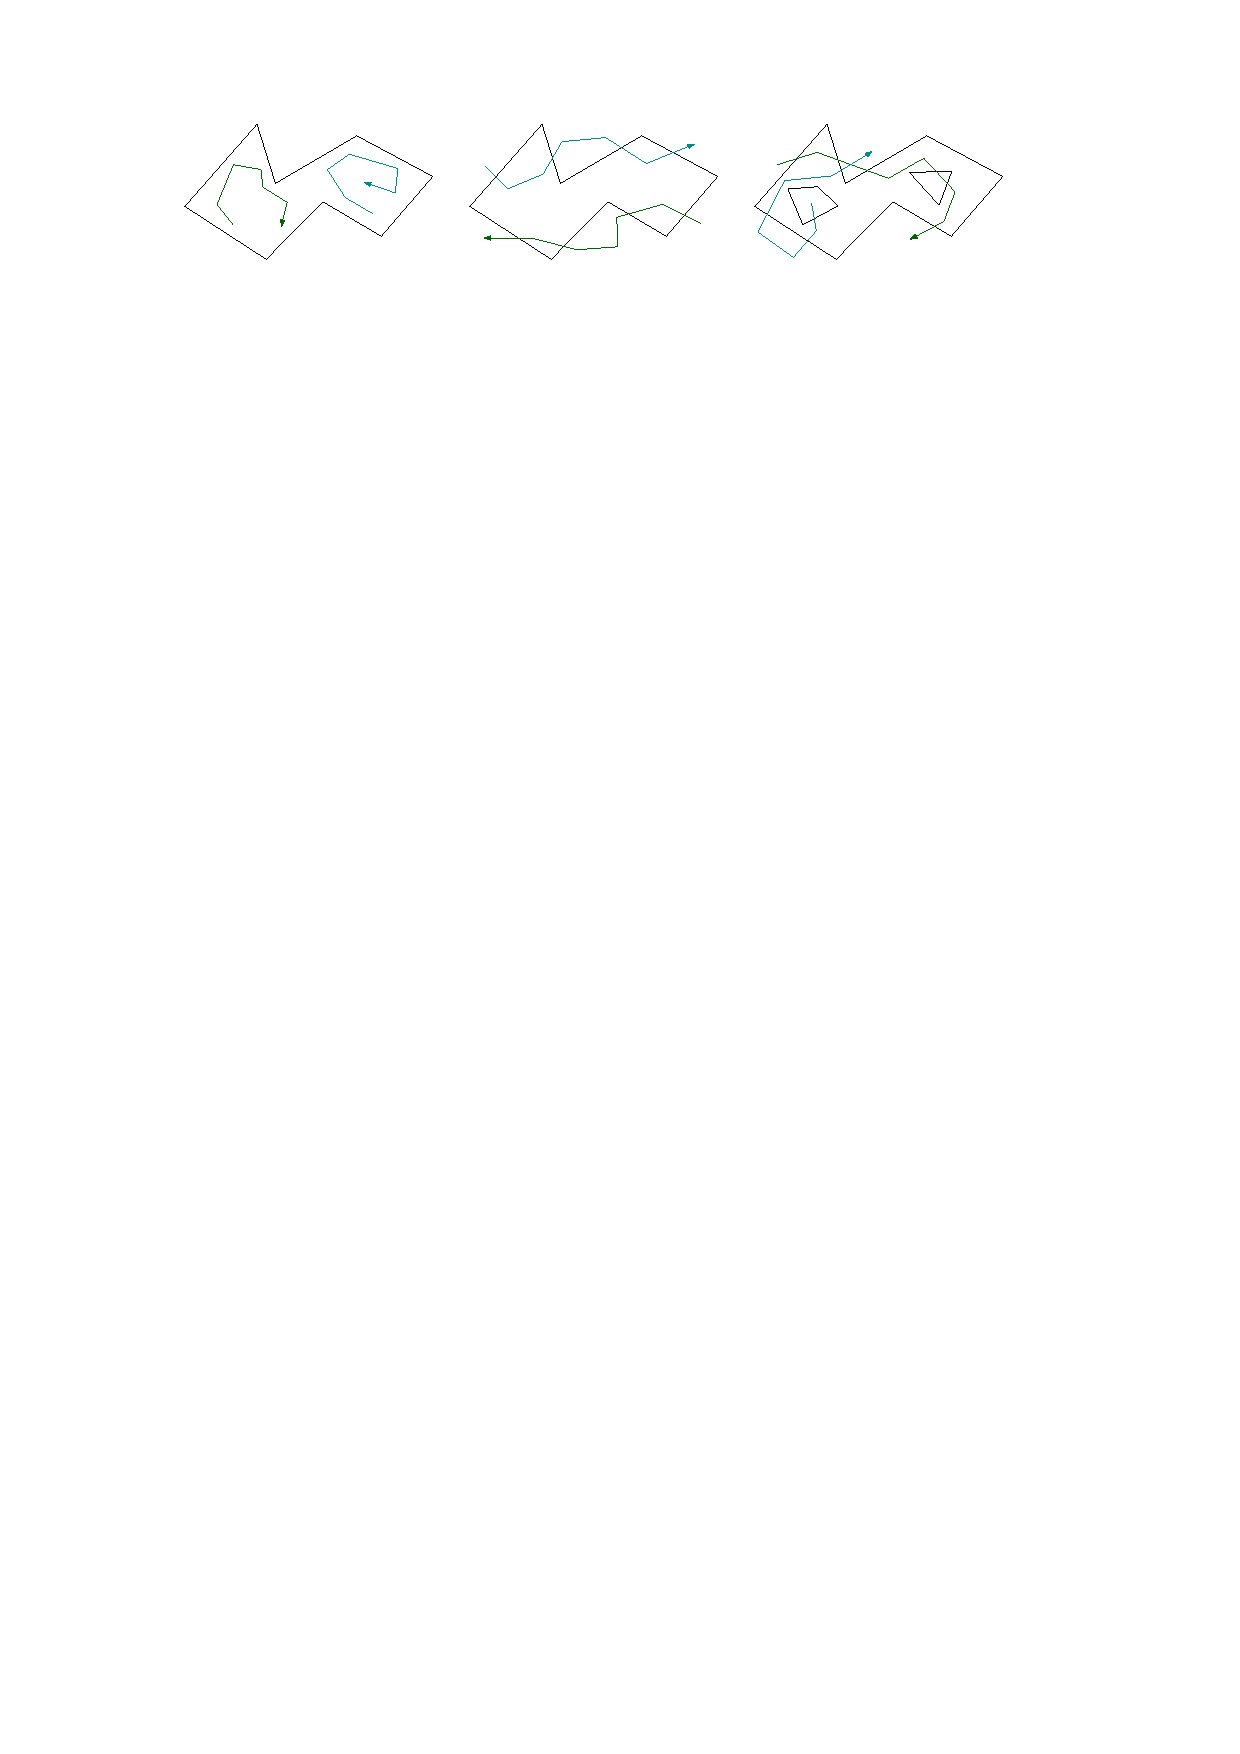
\includegraphics {variants} 
	\caption
	{
	  Different variations of the problem:
	  two trajectories inside a simple polygon (left);
	  two trajectories intersecting a simple polygon (middle);
	  or two trajectories in a polygonal domain (right).
	}  
	\addtolength{\belowcaptionskip}{-50pt}
	\label{fig:variants}
\end{figure}



In this paper, we study the following fundamental question, which we refer to as {\em trajectory visibility} testing.
  Given a simple polygon, or a polygonal domain, $P$, and the trajectories of two moving entities $q$ and $r$, is there a time $t$ at which $q$ and $r$ can see each other?
  We assume that $q$ and $r$ move linearly with constant (but possibly different) speeds between trajectory vertices, and cannot see though the edges of $P$.
  We distinguish several variants depending on whether $P$ is a simple polygon or a polygonal domain, and whether the trajectories are allowed to intersect $P$ (e.g. vehicles moving through fog, animals moving though foliage) or not (e.g. pedestrians moving among buildings, ships moving on water bodies). Refer to Figure~\ref {fig:variants}.
  We further consider the same variants in the simpler scenario in which one of the entities is a point (e.g. a stationary guard and a moving intruder).
%
%Part of the reason may be that studying trajectories in {\em context} is still relatively new area, and context is essential for meaningful question.
%On the other hand, the role of {\em time} is essential in this scenario: we are not interested whether there exists visibility between two geometric shapes, but rather whether there exists a {\em time} at which two point objects are visible. This makes the question fundamentally different from existing work in visibility.

Note that we are only interested in whether there {\em
  exists} a time at which the two entities see each other. % (more complex questions may be considered, we start with the most basic version; refer also to Section~\ref {sec:conclusions}).
This implies we can temporaly decompose the problem: the answer is {\em no} if and only if the answer is no between all two consecutive time stamps.
When considering this question, two fundamentally different approaches come to mind.
On the one hand, when the number of trajectory vertices $\tau$ is small compared to the number of polygon vertices $n$, the best approach may be to simply solve the problem for each time interval separately. 
On the other hand, when $\tau$ is large compared to $n$, it may be more efficient to spend some time on preprocessing $P$ first, if this allows us to spend less time per trajectory edge.
We therefore distinguish between the {\em algorithmic} and the {\em data structure} question. 
%\maarten {In the full version, we should also define the algorithmic problem of finding optimal dependence on $n$ and $\tau$.}


\subparagraph {Related work on visibility for moving entities.}

Somewhat surprisingly, given the amount of research on both trajectories and visibility, not much previous work exists on their combination.
%Visibility of a moving object is an old subject that recently has gained attention within the computational geometry community. 
Bern \etal~\cite{bern1994visibility} and  Mulmuley \cite{mulmuley1991hidden} study maintaining the visibility polygon of a point that moves over a straight path. 
Aronov \etal~\cite{aronov2002visibility} demonstrate a kinetic algorithm that tracks the visibility polygon of a moving query point $q$. The most recent result on visibility and motion is by Diez \etal~\cite{DKRRS2017KineticAPSPEuroCG} who show how to maintain the shortest path between two moving entities using a kinetic data structure. $q$ and $r$ are mutually visible if and only if their shortest path is a line segment, however as $q$ and $r$ traverse their trajectory there might be a linear number of kinetic events. A large body of work exists on the complementary problem of planning trajectories under visibility constraints~\cite{6907405}.




\newcolumntype{Y}{>{\centering\arraybackslash}X}
\begin{table}[t]
    \centering
    \begin{tabularx}{\linewidth}{ccYYYYYY}
      \toprule
      $q$ & $r$ & $P$ & algorithm & \multicolumn{3}{c}{data structure} & source \\
          &     &     &           & space & preprocessing & query & \\
        \midrule
        %
        $\bullet$ & $\bullet$ & S or I &  $\Theta(n)$ & $\O(n)$ & $\Theta(n)$ & $\Theta(\log n)$ & \cite{guibas1989optimal} \\
                  &           & D      & $\Theta(n)$ & $\mathcal{O}(n^2)$ & $\mathcal{O}(n^2)$ & $\Theta(\log n)$ & \cite{POCCHIOLA1996279}
        \\[0.6em]
        %
        $\bullet$ & $\slash$ & S & $\Theta(n)$ & $\O(n)$ & $\mathcal{O}(n \log n)$ & $\Theta(\log n)$ & Section~\ref{sec:pointline} \\
                  &          & I & $\mathcal{O}(n \log n)$ & $\mathcal{O}(n^{2} \log^3 n)$ & $\mathcal{O}(n^{2}\log^3 n)$ & $\mathcal{O}(n^{\frac{3}{4}+\varepsilon})$ & Section~\ref{sec:pointline} \\
                  &          & D & $\Theta(n \log n)$ & $\mathcal{O}(n^4 \log^3 n)$ & $\mathcal{O}(n^{4} \log^3 n)$ & $\mathcal{O}(n^{\frac{3}{4} + \varepsilon})$ &  Section~\ref{sec:pointline}
        %
        \\[0.6em]
        $\slash$ & $\slash$ & S & $\Theta(n)$ & $\mathcal{O}(n \log^5 n)$ & $\mathcal{O}(n^{1}\log^5 n)$ & $\mathcal{O}(n^{\frac{3}{4}}\log^2 n)$ & Section~\ref{sec:lineline} \\
                 &          & I & $\mathcal{O}(n \log n)$ & $\mathcal{O}(n^{3k})$ & $\mathcal{O}(n^{3k})$ & $\mathcal{O}(\log^k n)$ & Section~\ref{sub:Polygonal_Domain}  \\
                 &          & D & $\Theta(n \log n)$ & $\mathcal{O}(n^{3k})$ & $\mathcal{O}(n^{3k})$ & $\mathcal{O}(\log^k n)$ & Section~\ref{sub:Polygonal_Domain} \\
        \bottomrule
    \end{tabularx}
        \caption{Results using partition trees. The two left-most
          columns specify if the query entity is a point ($\bullet$)
          or line segment ($\slash$). The third column specifies if
          the domain $P$ is a simple polygon (S), a polygon where the
          query segments may intersect $P$ (I) or a polygonal domain
          with $n$ vertices (D). In the last rows, $k$ is an unspecified constant. 
        }
    \label{tab:results}
    %\vspace{-20pt}
\end{table}

\subparagraph {Our Results.}
  We focus on trajectories of at most two vertices.
  Our results are summarized in Table~\ref {tab:results}.
 %
  In Section~\ref{sec:oneshots}, we discuss our algorithmic results; we build on the geometric structure from this section in the remainder of the paper.
  In Section~\ref{sec:prelims} we consider the sub-problem of preprocessing a convex polygon $P'$ for intersection queries with quadratic curve segments.
  We then extend the solution in Section~\ref{sec:lineline} to a data structure for preprocessing $P$ using multi-level data structures. 
  In Section~\ref{sec:variants}, we sketch our solutions to the remaining variants of the problem.
  In Section~\ref{sub:Polygonal_Domain}, we investigate the degree in which our solution from Section~\ref{sec:lineline} can be extended to the cases where $P$ is a polygonal domain. The techniques are similar but the resulting data structure requires much more space.
  In Section~\ref{sec:pointline}, we study the more restricted problem in which one of the entities is stationary. We show that these problems can be solved with a different approach that is more efficient.

  Due to space constraints, several proofs and the full description of all results is deferred to the appendix.

\section{An algorithm for testing visibility}
\label{sec:oneshots}

Let $P$ be a polygonal domain with $n$ edges and $q$ and $r$ be two line segments in the plane (possibly of length 0). We first present an $\O(n\log n)$ time algorithm to solve the visibility problem for $q,r$ and $P$ and we show this algorithm is tight in the worst case. Finally, we show how to solve the visibility problem in linear time in the case where $P$ is a simple polygon and $q$ and $r$ are contained in $P$.

\subparagraph{An $O(n \log n)$ time algorithm.}
The entities $q$ and $r$ each move along a line segment with constant speed (depending on the length of the line segment) during the time interval $[0,1]$.\footnote {With slight abuse of notation, we use $q$ and $r$ to refer to both the (moving) entities and their trajectory.}
Consider the line $g(t)$ through the entities at time $t$.
We dualize this line to a point using classical point-line dualization (i.e. we map the line $y = ax + b$ to the point $(a, -b)$); this point now traces a segment of a curve $\gamma : [0,1] \to \R^2$ in the dual space.\footnote {Throughout this paper we follow the convention of using latin letters for objects in primal space and greek letters for their duals.}

\begin{lemma}
  \label{lemma:hyperbola}
  The segment $\gamma$ is a segment of a hyperbolic curve with $5$ degrees of freedom.
\end{lemma}

Let $e$ be an edge of $P$ and denote by $L_e$ the set of lines intersecting $e$. 
The dual of $L_e$ is a {\em wedge} $\Lambda_e$~\cite{de1997computational}. If the segment between $q$ and $r$ is blocked by $e$ at time $t$ then $g(t)$ must lie in $L_e$. 
In the dual, this means that the curve segment $\gamma$ must intersect $\Lambda_e$.
There are at most two connected time intervals where a quadratic curve segment $\gamma$ can intersect a wedge $\Lambda_e$; it follows that each edge $e$ has at most two connected time intervals where it blocks the visibility between $q$ and $r$.
This leads to a straightforward general algorithm to test if there is a time at which $q$ can see $r$: for each edge $e \in P$, we compute the at most two time intervals where it blocks visibility between $q$ and $r$ in constant time. 
We sort these time intervals in $\O(n \log n)$ time and check if their union covers the time interval $[0,1]$.

\begin{figure}[h]
    \centering
    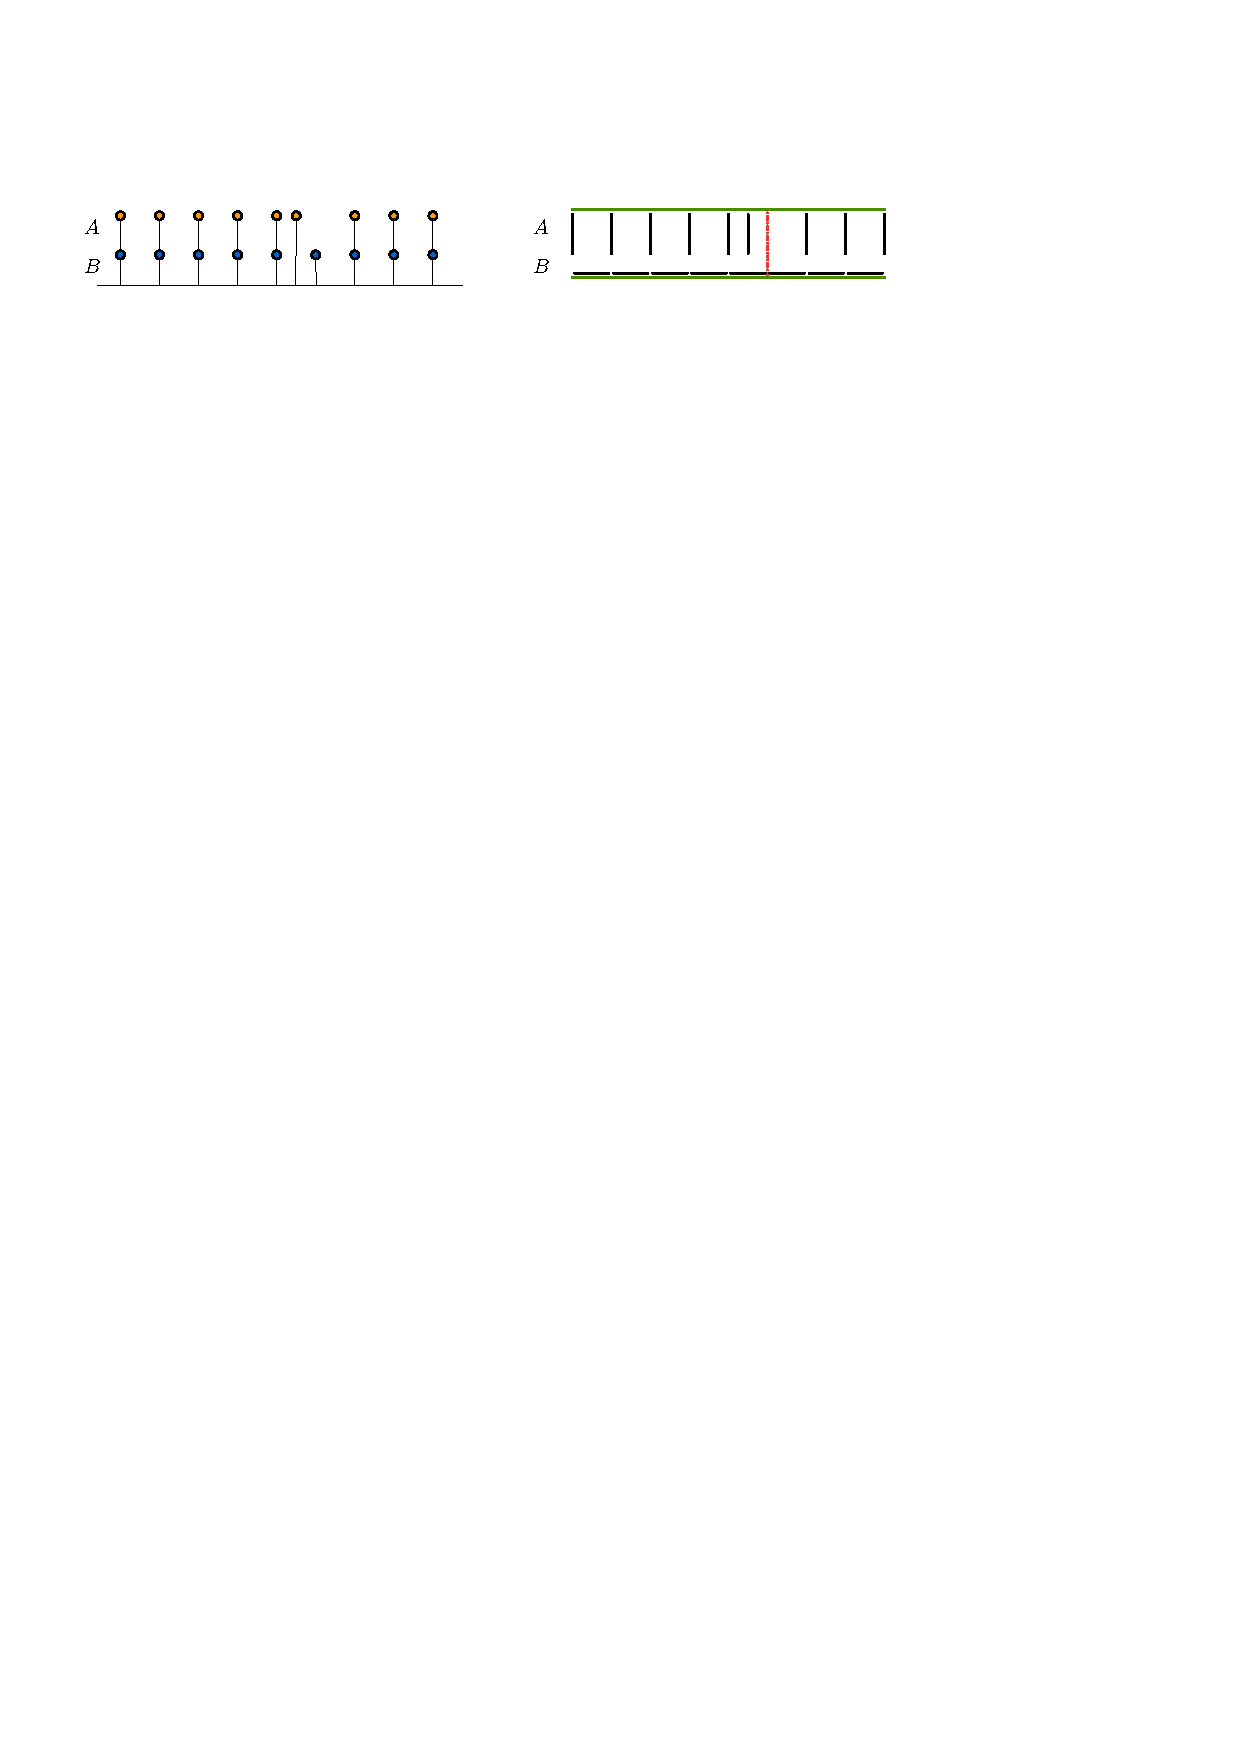
\includegraphics{../reduction}
    \caption{The reduction for when $P$ is a polygonal domain with $\Omega(n)$ holes.}
    \label{fig:reduction}
\end{figure}

\begin{theorem}
  \label{thm:algorithm_general}
  Given a polygonal domain $P$ with $n$ vertices and moving entities $q$ and $r$, we can test trajectory visibility in $\mathcal{O}(n \log n)$ time.
\end{theorem}

\subparagraph{An $\Omega(n \log n)$ lower bound.}
If $P$ is a polygonal domain with $\Omega(n)$ holes, this result is tight: suppose we are given a set of $n$ numbers $A$ and we want to know if $A = B$ for a given arbitrary sorted set $B = \{x_1,x_2, \ldots x_n \}$. 
Ben-Or~\cite{ben1983lower} shows that this problem has an $\Omega(n \log n)$ lower bound in the algebraic decision tree model. 
This leads to the following reduction (illustrated in Figure~\ref{fig:reduction}): we construct a set of $n$ horizontal edges whose $y$-coordinates are $0$ and whose $x$-coordinates are $\{ (x_{i} - \varepsilon, x_{i+1} + \varepsilon ) \mid i \in [1, n-1] \}$ where $\varepsilon$ is smaller than the minimal difference between two consecutive numbers in $B$, a value for $\varepsilon$ can be found in linear time since $B$ is sorted.
For each of the $n$ numbers $x \in A$ we construct the vertical edge from the point $(x, 1)$ to $(x,2)$ with a width of $\varepsilon$. 
The entity $q$ walks from the point $(1,-1)$ to $(n, -1)$ and entity $r$ walks from $(1,3)$ to $(n, 3)$. 
Suppose the number $x_j$ from $B$ is not in $A$, then $q$ can see $r$ at the $x$-coordinate $x_j$. 
Note that this construction also extends to the case where one of the two entities is stationary: consider the cone between the stationary entity $q$ and a horizontal line segment trajectory $r$: we can transform the set $B$ into a set of $n$ horizontal edges that cut in the cone between $q$ and $r$. 
Each number $x \in A$ gets transformed not to a vertical edge, but an edge that lies on a ray from $q$ to $r$.



\begin{theorem}
    Given a polygonal domain $P$ with $n$ vertices and moving entities $q$ and $r$, testing trajectory visibility has an $\Omega(n \log n)$ time lower bound.
\end{theorem}


\subparagraph{A linear-time algorithm for when $P$ is a simple polygon and
  $q,r \subset P$.}  Any segment between $q$ and $r$ that is contained in $P$
is the shortest path in $P$ between those two points on $q$ and $r$. Guibas and
Hershberger~\cite{guibas1989optimal} define for any two segments $q$ and $r$ in
a simple polygon $P$, the \emph{hourglass} $H(q,r)$ to be the union of all
shortest paths between points on $q$ and $r$. The hourglass $H(q,r)$ is a subset of $P$
and bounded by the segments $q$ and $r$ and by two shortest paths.
The {\em ``upper'' chain} is the shortest path between the upper end points $p_q^+$ $p_r^+$ of $q$ and $r$,
and the {\em ``lower'' chain} is the shortest path between $p_q^-$ and $p_r^-$ (refer to Figure~\ref{fig:visibilityglass}). 
We define the \emph{visibility glass} $L(q,r)$ as the (possibly
empty) union of \emph{line segments} between $q$ and $r$ that are
contained in $P$. Notice that $L(q,r)$ is a subset of $H(q,r)$.
 
  
 \begin{figure}[h]
    \centering
    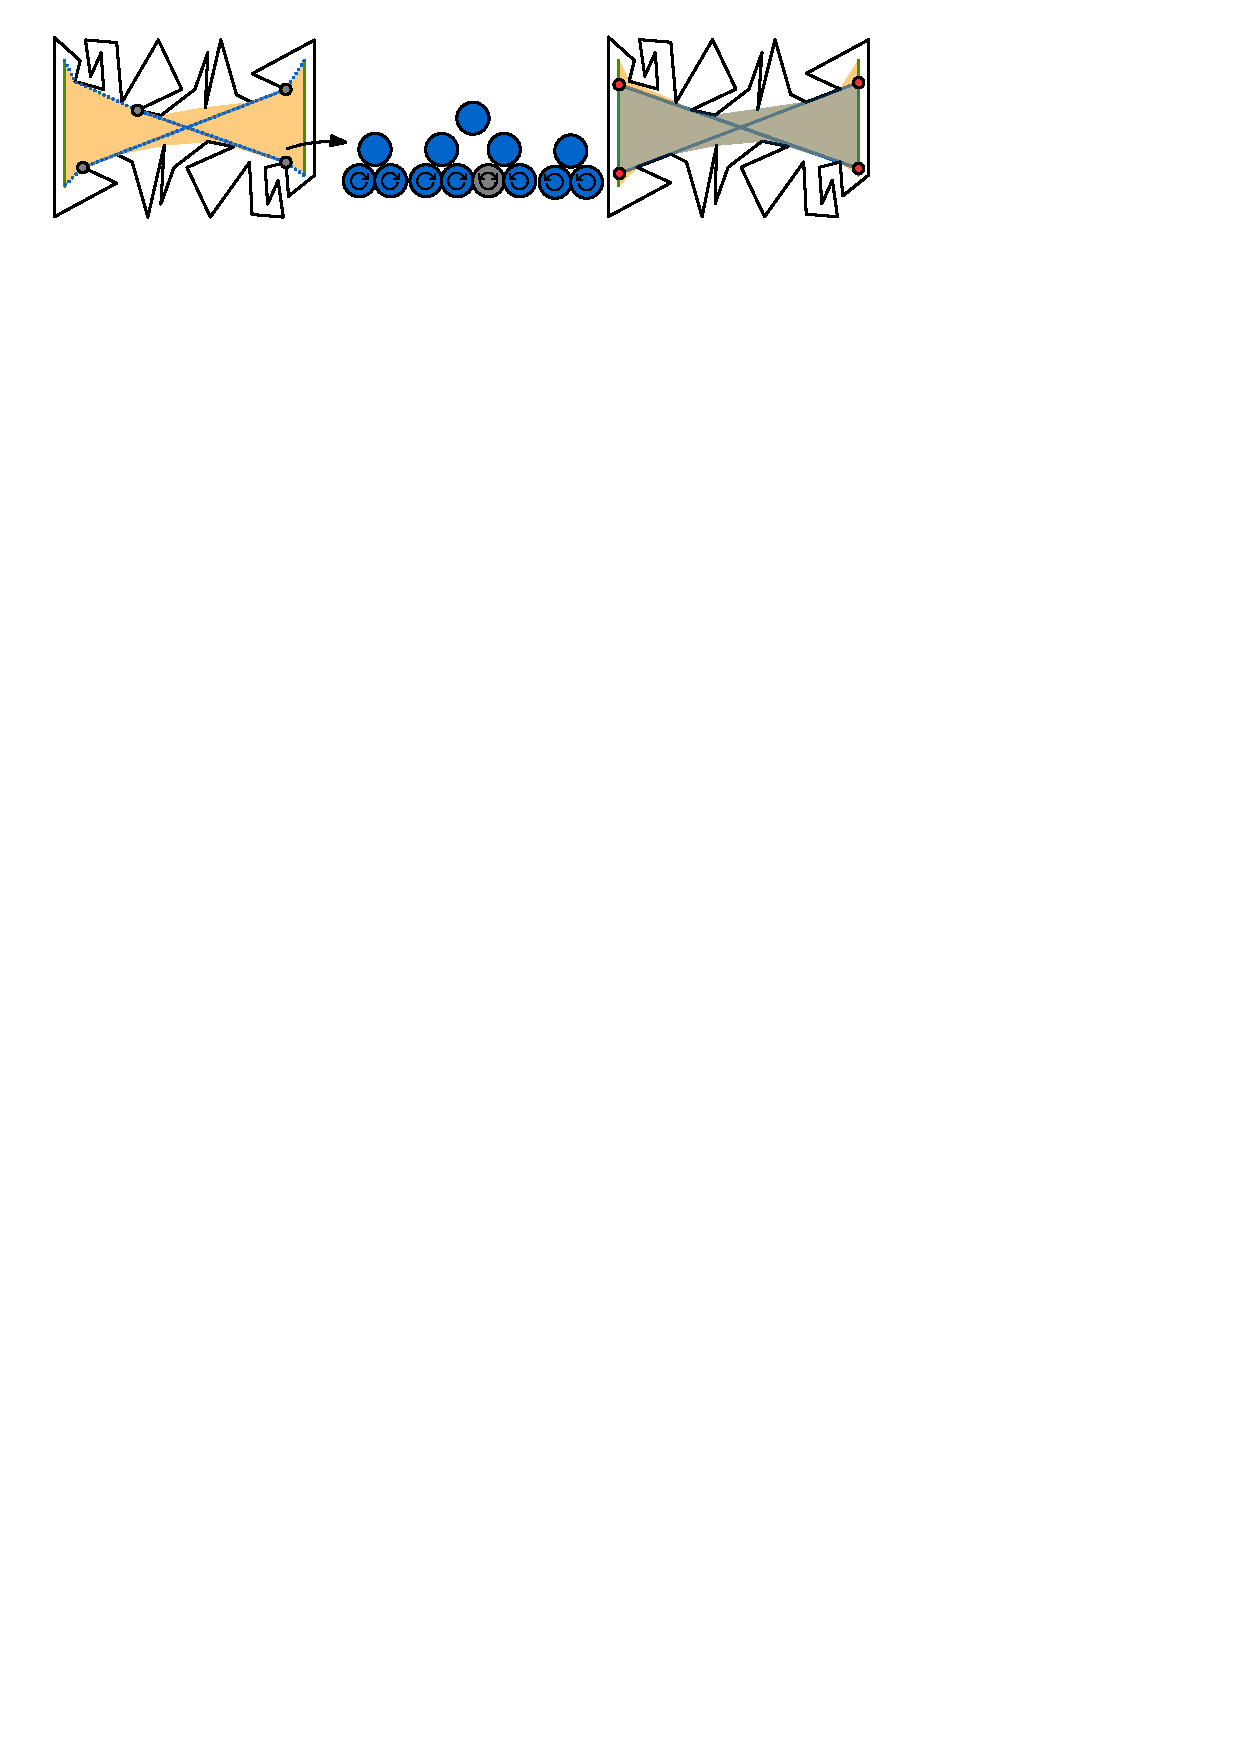
\includegraphics[]{../visibilityglass}
    \caption{(left) $H(q,r)$ in orange. The path from $p_q^+$ to $r_q^-$ shown  as a dotted path. (middle) only the bitangent on this path starts in clockwise and ends in counterclockwise rotation. (right) Using the bitangents, we identify the endpoints of $q'$ and $r'$ and obtain $L(q,r)$ in grey. \ivor{make convex homepc}}
    \label{fig:visibilityglass}
\end{figure}

 

 
\begin{observation}
  \label{obs:obtain_L}
  For any two segments $q, r \in P$, there exist segments
  $q' \subset q, r' \subset r$ s.t. $L(q, r) = H(q', r')$. Moreover, $q'$ and
  $r'$ are bound by two bitangents on the shortest paths between the endpoints of $q$ and $r$.
\end{observation}

\begin {proof}
Suppose that the upper and lower chain of $H(q,r)$ share a vertex. Then the visibility glass $L(q,r)$ is either a single segment or empty and thus we can either find two points $q'$ and $r'$ on $q$ and $r$ whose line segment forms $H(q', r') = L(q,r)$ or $q'$ and $r'$ are empty. 

If the upper and lower chain do not share a vertex then these chains are semi-convex~\cite{guibas1989optimal}. Consider the path from $p_q^+$ to $p_r^-$, this path has one edge $(u,v)$ connecting the upper and lower chain. This is the unique edge for which the path makes a clockwise turn at $u$ and a counterclockwise turn at $v$ or vice versa. Consider the corresponding edge that we obtain from the path between $p_q^-$ and $p_r^+$. The extension of these edges bound $q'$ and $r'$~\cite{Chazelle1989}.
\end {proof}


Chazelle and Guibas~\cite{Chazelle1989} note that (the supporting lines of) all
line segments in $L(q,r)$ can be dualized into a convex polygon of linear
complexity which we denote by $\Lambda(q,r)$.\footnote {If $L(q,r)$ contain vertical lines, it will dualize into a pair of unbounded convex regions. For simplicity of exposition, we assume this is not the case; our results can be adapted to deal with degeneracies.}
A shortest path between two points in
$P$ can be computed in linear time~\cite{GuibasHLST87}. Finding the bitangents also takes linear time. It follows that we can compute $L(q,r)$ and its dual $\Lambda(q,r)$ in linear time.
Suppose we are given two entities $q$ and $r$ that each traverse a line segment in a simple polygon $P$. 
We noted earlier that the line $g(t)$ through $q$ and $r$ traces a hyperbolic segment $\gamma$ in the dual.

\begin{observation}
  \label{obs:visible}
  Entities $q$ and $r$ are mutually visible at time $t$ if
  $\gamma(t)$ lies in $\Lambda(q,r)$.
\end{observation}
\begin {proof}
The entities can see one another at time $t$ if and only if $g(t) \in L(q,r)$.
\end {proof}



We can derive $\gamma$ in constant time, construct $\Lambda(q,r)$ in linear time, and we can check if a quadratic curve intersects a convex polygon in linear time. Thus we conclude:

\begin{theorem}
  \label{thm:algorithm_simple_polygon}
  Given a simple polygon $P$ with $n$ vertices and two entities $q$ and $r$
  moving linearly inside $P$, we can test trajectory visibility in $\Theta(n)$ time.
\end{theorem}





  
\section{Intersecting a convex polygon with an algebraic curve}
\label{sec:prelims}
We now turn our attention to the data structure question: can we preprocess $P$ such that trajectory visibility may be tested efficiently (i.e. in sublinear time) for a {\em query} pair of segments $q$, $r$.
By Observation~\ref {obs:visible}, we know that we may phrase such a query as an intersection between a hyperbolic curve segment and a convex polygon.
Note, however, that both the curve segment and the convex polygon depend on the query segments $q$ and $r$.
As an intermediate step, we study a simplified problem in this section, which we believe to be of independent interest;
we will use the solution to this question as a subroutine in Section~\ref {sec:lineline}.
Let $P'$ be a convex polygon with $n$ edges. Is it possible to preprocess $P'$ such that for any quadratic curve segment $\gamma$, we can quickly test if $\gamma$ intersects $P'$? 


\subparagraph{Semi-algebraic range searching.}  Let $X$
be a set of $n$ geometric objects in $\mathbb{R}^d$, where each object
is parametrized by a vector $\vec{x}$ (e.g. a point is parametrized by
a vector of its coordinates). Let $\Gamma$ be a family of geometric
regions (called semi-algebraic ranges) in $\mathbb{R}^d$ where each
region $G \in \Gamma$ is bound by an algebraic curve $\gamma$ which is
parametrized by a vector
$\vec{a}$. Agarwal~\etal~\cite{agarwal2013range} describe how to 
preprocess $X$, such that for any range $G \in \Gamma$, we can
efficiently count the number of objects of $X$ intersecting $G$. Let
$F$ be a function mapping (the parameterizations of) $x \in X$ and $G \in \Gamma$ to
$\R$ such that $F(\vec{x},\vec{a}) \leq 0$ if and only if $x$ and $G$
intersect.
Agarwal \etal show that if $F$ can be written in the form $F(\vec{x}, \vec{a}) = g_0(\vec{a}) + \sum_{i=1}^k g_i(\vec{a})f_i(\vec{x})$ (where $f_i$ and $g_i$ are polynomials dependant only on $\vec{x}$ and $\vec{a}$, respectively) then there is a function $f$ that maps the objects in $X$ to points in $\R^k$, and a function $g$ that maps the ranges in $\Gamma$ to halfspaces in $\R^k$, such that $f(x) \in g(G)$ if and only if $x$ intersects $G$. 
This so-called \emph{linearization} process transforms a $d$-dimensional semi-algebraic range searching problem into a halfspace range searching problem into $\mathbb{R}^k$.
Refer to Appendix~\ref{appx:introduction} for more information about algebraic range searching and examples.

The resulting set of $n$ points in $\R^k$ can be stored in a data structure of linear size such that the points in a query halfspace can be counted in $O(n^{1-\frac{1}{k}})$ time (with high probability)~\cite{chan2012optimal}.
Testing if a query halfspace is empty can be done in expected $O(n^{1-\frac{1}{k/2}})$ time. 
Data structures with a slightly slower deterministic query time are also
known~\cite{chan2012optimal}. 
If we are willing to use (much) more space, faster query times are also possible~\cite{chan2012optimal,Mat1993}.


\subparagraph{Semi-algebraic range searching and our intersection query.}
The $n$ edges of a simple polygon $P'$ are algebraic objects.
A natural parametrization for an arbitrary edge $e \in P'$ would be a 4-dimensional vector $\vec{x}_e$ specifying its start and end point. 
A quadratic curve segment $\gamma$ per definition is an semi-algebraic range parametrized by its own parameters $\vec{a}_\gamma$. 
If we want to apply semi-algebraic range searching, we need to design a predicate function $F(\vec{x}_e, \vec{a}_\gamma)$ that outputs a negative real number whenever the edge $e$ is intersected by $\gamma$. 

It is tempting to immediately construct such a predicate function using the parameters $\vec{x}_e$ and $\vec{a}_\gamma$ only (ignoring geometric facts such as the convexity or connectedness of $P'$). 
However, we have to linearize the resulting predicate function $F(\vec{x}_e, \vec{a}_\gamma)$ into $k$ terms. 
The more complex the description of the objects, the query and their intersection the more complex the predicate will be and therefore the higher this number $k$ will be.
In Appendix~\ref{sub:intersecting_line_segments_with_a_quadratic__curve_segment} (Lemma~\ref{lemma:15000}) we show that it is indeed possible to apply semi-algebraic range searching only in the parametrizations of an arbitrary edge $e$ and curve segment $\gamma$.
This transforms the intersection query between a set $E$ of $n$ \emph{arbitrary edges} and a degree-2 curve segment $\gamma$ into four consecutive halfspace emptyness problems in $\R^k$, where $k \approx 15 000$. 
While this leads to a linear-size data structure with sub-linear  %($O(n^{1-\frac{1}{15 000}})$) 
query time, we can do better.
%Instead, we employ an approach that we will use throughout this paper. We make several observations about the ways in which a convex polygon $P'$ can be intersected by a degree-2 curve. Many types of intersections can be detected using conventional geometric data structures. This leaves us with a more restricted case of an intersection between $\gamma$ and $P'$ that conventional data structures cannot find. Since this is a more restricted problem, it can be linearized to a much lower dimension ($\mathbb{R}^5$).

\subparagraph{Geometry of our intersection query.}

Let $P'$ be a simple polygon with $n$ edges. Let $\gamma$ be a quadratic curve segment ending in the points $s$ and $z$ and let $\Gamma$ denote the
unique degree-2 curve $\Gamma \supset \gamma$ given by
$a_1 x^2 + a_2 x + a_3 xy + a_4 y + a_5 y^2 + a_6 = 0$. We say 
$\vec{a} = (a_1, \ldots, a_6)$. Observe (Figure~\ref{fig:intersectionsearch}) that if $\gamma$ intersects
$P'$, then either (a) an endpoint $s$ or $z$ lies in $P'$, or (b) $\gamma$ cuts
off a vertex, or (c) $\gamma$ intersects only a single edge of $E$ twice and has no
endpoint in $P_E$ (we call this \emph{dipping}). Intersections of type $(a)$
and $(c)$ can be identified with a regular binary search on on $P'$. An
intersection of type $(b)$ is detected using algebraic range searching.
%
\begin{figure}[tb]
    \centering
    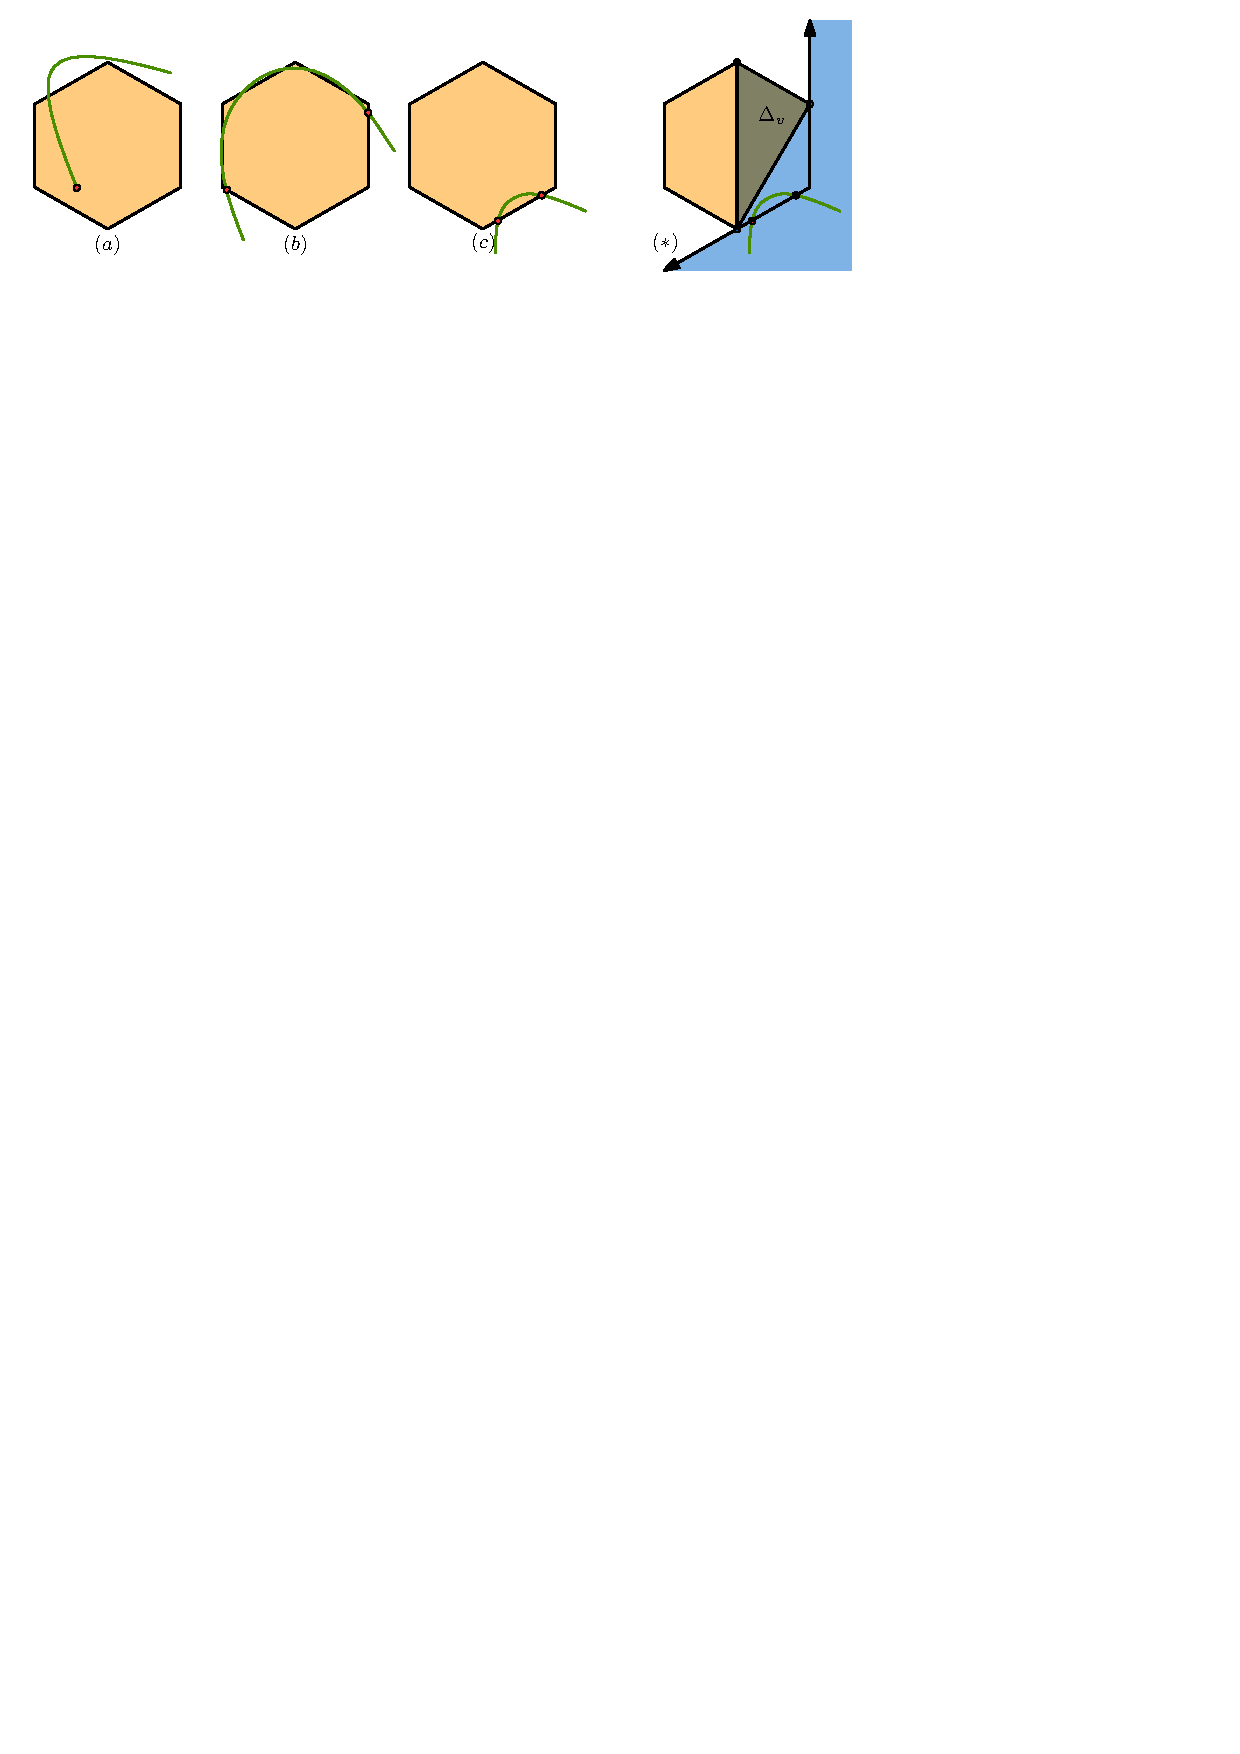
\includegraphics{../intersectionsearch}
    \caption{(left) The three cases of an intersection between $\gamma$ and $P_E$. (right) the right-subspace bound by three halfspaces.}
    \label{fig:intersectionsearch}
\end{figure}

Since $P'$ is convex, we can
test if an endpoint of $\gamma$ lies inside $P'$ in $O(\log n)$ time. To
detect an intersection of case $(c)$, we store a Dobkin-Kirkpatrick hierarchy~\cite{dobkin1983intersection} of $P'$. This takes $\O(n)$ space
and requires $\O(n)$ preprocessing time. Given $\gamma$, we detect an intersection of type $(c)$ as follows (Figure~\ref{fig:intersectionsearch} (*)):
any node $v$ in this decomposition represents a sub-polygon $P''$ of $P'$ and a
triangle $\Delta_v$ which splits $P''$ in a left and right part. Consider the
border of the right part $R = (e_1, e_2, \ldots, e_m)$. Note that if $\gamma$
does not intersect $\Delta_v$, then $\gamma$ can only dip an edge in $R$ if it
is contained in the union of the half-spaces that lie to the right of the lines
supporting (1) one edge of $\Delta_v$ and (2) $e_1$ and $e_m$ (refer to the
blue area in the figure). Given the node $v$ we do three constant
time checks. First we check if $\gamma$ intersects $\Delta_v$. If not then we
check for both the left and right sub-polygon if $\gamma$ is contained in the
specified area. If that is the case for both or neither sub-polygons then
$\gamma$ can never dip an edge of $P_E$, else we recurse. It follows that we
can detect case $(c)$ in $\mathcal{O}(\log n)$ time. 
\begin{lemma}
  We can preprocess a simple polygon $P'$ consisting of $n$ edges in $\mathcal{O}(n)$ time and using $\mathcal{O}(n)$ space, such that for any degree-2 curve segment $\gamma$ we can detect an intersection of type $(a)$ or $(c)$ in $\mathcal{O}(\log n)$ time.
\end{lemma}


The curve $\Gamma$ of which $\gamma$ is a segment divides the plane into two areas, $\Gamma^- := \{ a_1 x^2 + a_2 x + a_3 xy + a_4 y + a_5 y^2 + a_6 \le 0  \}$ and its complement $\Gamma^+$. An edge $(x_1, x_2) \times (x_3, x_4)$ of $P'$ is intersected by $\gamma$ with an intersection of type $(b)$ only if one endpoint of the edge lies in $\Gamma^-$ and the other in $\Gamma^+$. If $\Gamma$ is a curve with $k+1 \le 6$ degrees of freedom then the formulation of $\Gamma^-$ and $\Gamma^+$ is a predicate that specifies whenever a point $\vec{x} = (x_1, x_2)$ lies in $\Gamma^-$ or $\Gamma^+$ with $k$ terms depending on variables from $\vec{x}$. This transforms the question of whether an edge has two points on either side of $\Gamma$ into two consecutive halfspace range queries in $\mathbb{R}^k$. 
We build a three-level data structure where the first two levels are
5-dimensional partition trees. On top of each node in the second level
we build a binary tree on the clockwise ordering (with respect to $P'$) of the edges in that node. 

During query time, we transform the degree-2 curve $\Gamma$ into two
$k$-dimensional halfspaces $g(\Gamma^+)$ and $g(\Gamma^-)$. With two
consecutive halfspace range queries we obtain the edges which have an
endpoint on either side of $\Gamma$ in $\mathcal{O}(n^ {1 -
  \frac{1}{k}})$ time. The result consists of $\mathcal{O}(n^ {1 -
  \frac{1}{k}})$ nodes in the secondary trees. For each such node we query
the associated binary search tree $T_i$: the subset of these edges
which are intersected by the segment $\gamma$ must be a consecutive subset of the leaves of $T_i$. 
Thus using $T_i$ we can obtain these consecutive leaves in $\mathcal{O}(\log n)$ time by checking testing if $\gamma$ lies before or after the point of intersection between $\Gamma$ and an edge in $T_i$.
The time and space needed for detecting case $(b)$ dominates the time and space needed for case $(a)$ and $(c)$ and we conclude:

\begin{theorem}
  \label{thm:intersect_convex_polygon}
  Let $P'$ be a convex polygon with $n$ vertices. In $\O(n\log^2 n)$ time we can
  build a data structure of size $\O(n\log^2 n)$ with which we can test if an
  arbitrary degree-2 query curve segment $\gamma$ with $k+1 \le 6$ degrees of freedom
  intersects $P'$ in $\O(n^{1 - \frac{1}{k-1}}\log n)$ time.
\end{theorem}




\section{A data structure for two entities moving inside a simple polygon}
\label{sec:lineline}

% \subsection{Curve-segment intersection queries with a convex polygon}
% \label{sub:A_data_structure_for_testing_intersections_between_a_curve_segment_with_a_convex_polygon}

In this section we build a data structure to answer trajectory visibility
queries in case both the entities $q$ and $r$ move linearly, possibly at
different speeds, inside a simple polygon $P$. Our main approach is the same as
in our algorithm from Theorem~\ref{thm:algorithm_simple_polygon}: we obtain the
convex polygon $\Lambda(q,r)$ that is the dual of the visibility glass
$L(q,r)$, and test if the curve segment $\gamma$ tracing the line through $q$
and $r$ in the dual space intersects $\Lambda(q,r)$. By
Observation~\ref{obs:visible} this allows us to correctly answer trajectory
visibility queries. The main challenge is that we cannot afford to construct
$\Lambda(q,r)$ explicitly. Instead, our data structure will allow us to obtain
a compact representation of $\Lambda(q,r)$ that we can query for intersections
with $\gamma$.


\begin{figure}[tb]
    \centering
    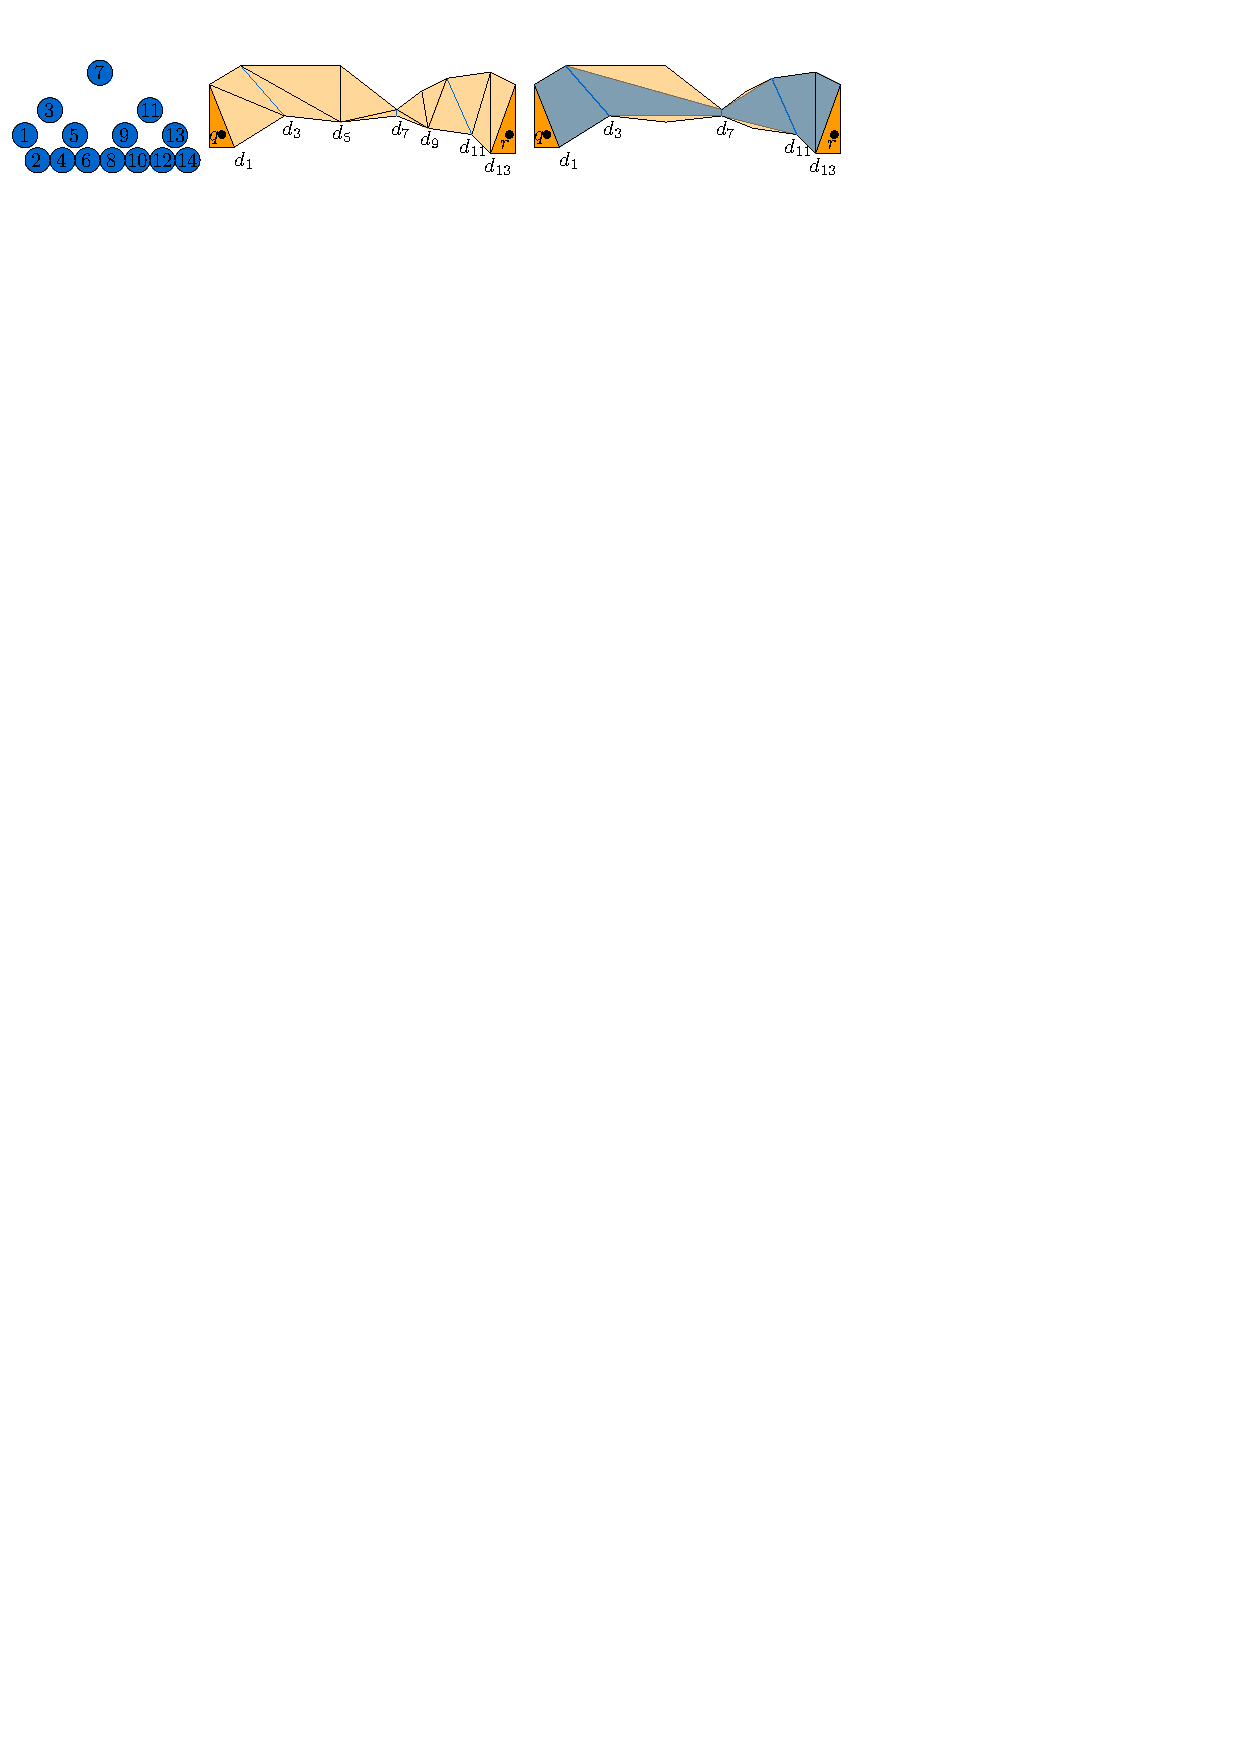
\includegraphics{../guibas}
    \caption{A triangulated polygon $P$ where the diagonals are labelled from $d_1$ to $d_{14}$. (left) a balanced hierarchical subdivision on the diagonals. In each node, G\&H store an hourglass between diagonals. (right) There are $13$ diagonals between $q$ and $r$. However, we have pre-stored hourglasses $H(d_1,d_3)$, $H(d_3, d_7)$, $H(d_7, d_{11})$ and $H(d_{11}, d_{13})$. During query time, we only have to concatenate these $\mathcal{O}(\log n)$ hourglasses to get $H(d_1, d_{13})$. }
    \label{fig:guibas}
\end{figure}

To obtain $\Lambda(q,r)$ we use a variation of two-point shortest-path query
data structure of Guibas and Hershberger~\cite{guibas1989optimal}. Their data
structure (Figure~\ref{fig:guibas}) compactly stores a collection of hourglasses that can be concatenated
to obtain a shortest path between two arbitrary points $p,p' \in P$. All
shortest paths, so in particular the boundary of the hourglasses, are
represented using balanced binary search trees storing the vertices on the
path. Guibas and Hersberger show that by reusing shared subtrees these $O(n)$
hourglasses can be stored using only $O(n)$ space. To report the shortest path
between two query points their data structure concatenates $O(\log n)$ of these
hourglasses. The result is again represented by a balanced binary tree.

Unlike the Guibas and Hershberger structure, we store the hourglasses
explicitly. In particular, the vertices on the boundary of an hourglass are
stored in the leaves of a balanced binary search tree. The internal nodes of
these trees correspond to semi-convex subchains. Let $T$ denote the collection
of all these nodes. Each node $v \in T$ stores its subchain $C_v$ in an
associated data structure. Specifically, we dualize the supporting-lines of the
edges in $C_v$ to points. Two consecutive edges produce two points in the dual, which we
again connect into semi-convex polygonal chains. 
So for every vertex in the sub-chain $C_v$ the associated data
structure $\Delta_v$ actually stores a line-segment; together these segments
again form a polygonal chain $\Psi_v$. The associated data structure will
support intersection queries with a hyperbolic query segment $\gamma$;
i.e.~it will allow us to report the segments of $\Psi_v$ intersected by
$\gamma$. We implement $\Delta_v$ using the data structure from
Theorem~\ref{thm:intersect_convex_polygon}. Refer to Figure~\ref{fig:panel} for an overview of this approach.

\begin{lemma}
  \label{lem:space_dual_chains}
  The total size of all chains $\Psi_v$ over all nodes $v$ is $O(n\log^3 n)$.
\end{lemma}

\begin{proof}
  The Guibas and Hershberger data structure is essentially a balanced
  hierarchical subdivision that recursively partitions the polygon into two
  roughly equal size subpolygons. Every subpolygon has $O(\log n)$
  diagonals~\cite{guibas1989optimal}, and thus stores at most $O(\log^2 n)$
  hourglasses\footnote{We use the version of Guibas and Hersberger's structure
    that achieves only $O(\log^2 n)$ query time.}. It follows that all
  hourglasses of a subpolygon of size $m$ have use at most $O(m\log^2 n)$
  space. The height of the balanced hierarchical subdivision is $O(\log n)$,
  and at every level the total size of the subpolygons is $O(n)$. Therefore,
  the total size of all subpolygons is $O(n\log n)$. The lemma follows.
\end{proof}

For a chain of size $m=|\Psi_v|$ the data structure $\Delta_v$ has size
$O(m\log^2 m)$ and can be built in $O(m\log^2 m)$ time. It follows that our
data structure uses $O(n\log^5 n)$ space in total, and can be built in
$O(n\log^5 n)$ time.

\begin{figure}[tb]
    \centering
    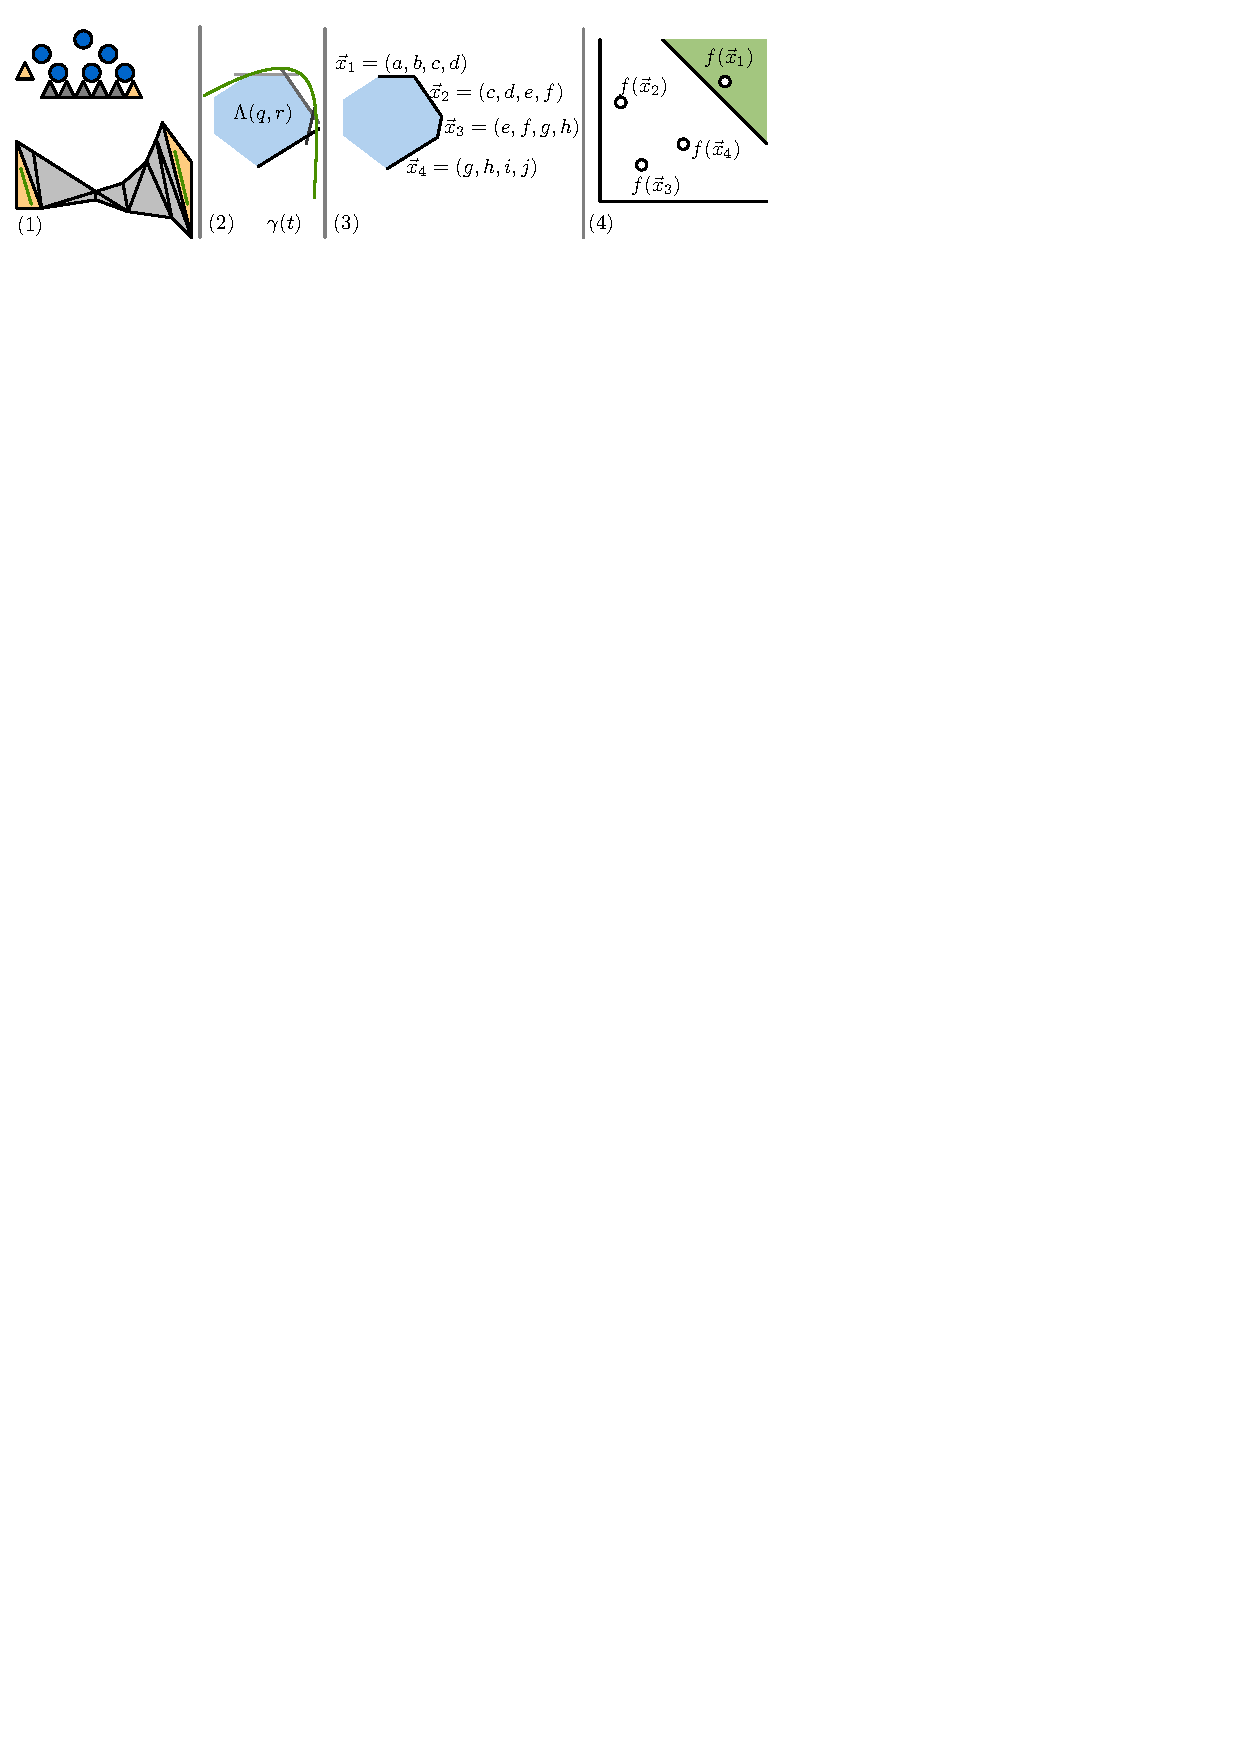
\includegraphics[]{../panel}
    \caption{(1) The base level of our data structure is a hierarchical
      triangulation. (2) Given $q$ and $r$, we compute $\Lambda(q,r)$ and the
      degree-2 curve segment $\gamma$. (3) We store the parameters of each edge
      of $\Lambda(q,r)$ (4) Each parameter vector gets mapped to a point in
      $\mathbb{R}^4$ and the query curve segment gets mapped to a 4-dimensional
      halfspace which is empty only if $\gamma$ intersects no edge from
      $\Lambda(q,r)$.}
    \label{fig:panel}
\end{figure}


\begin{figure}[tb]
    \centering
    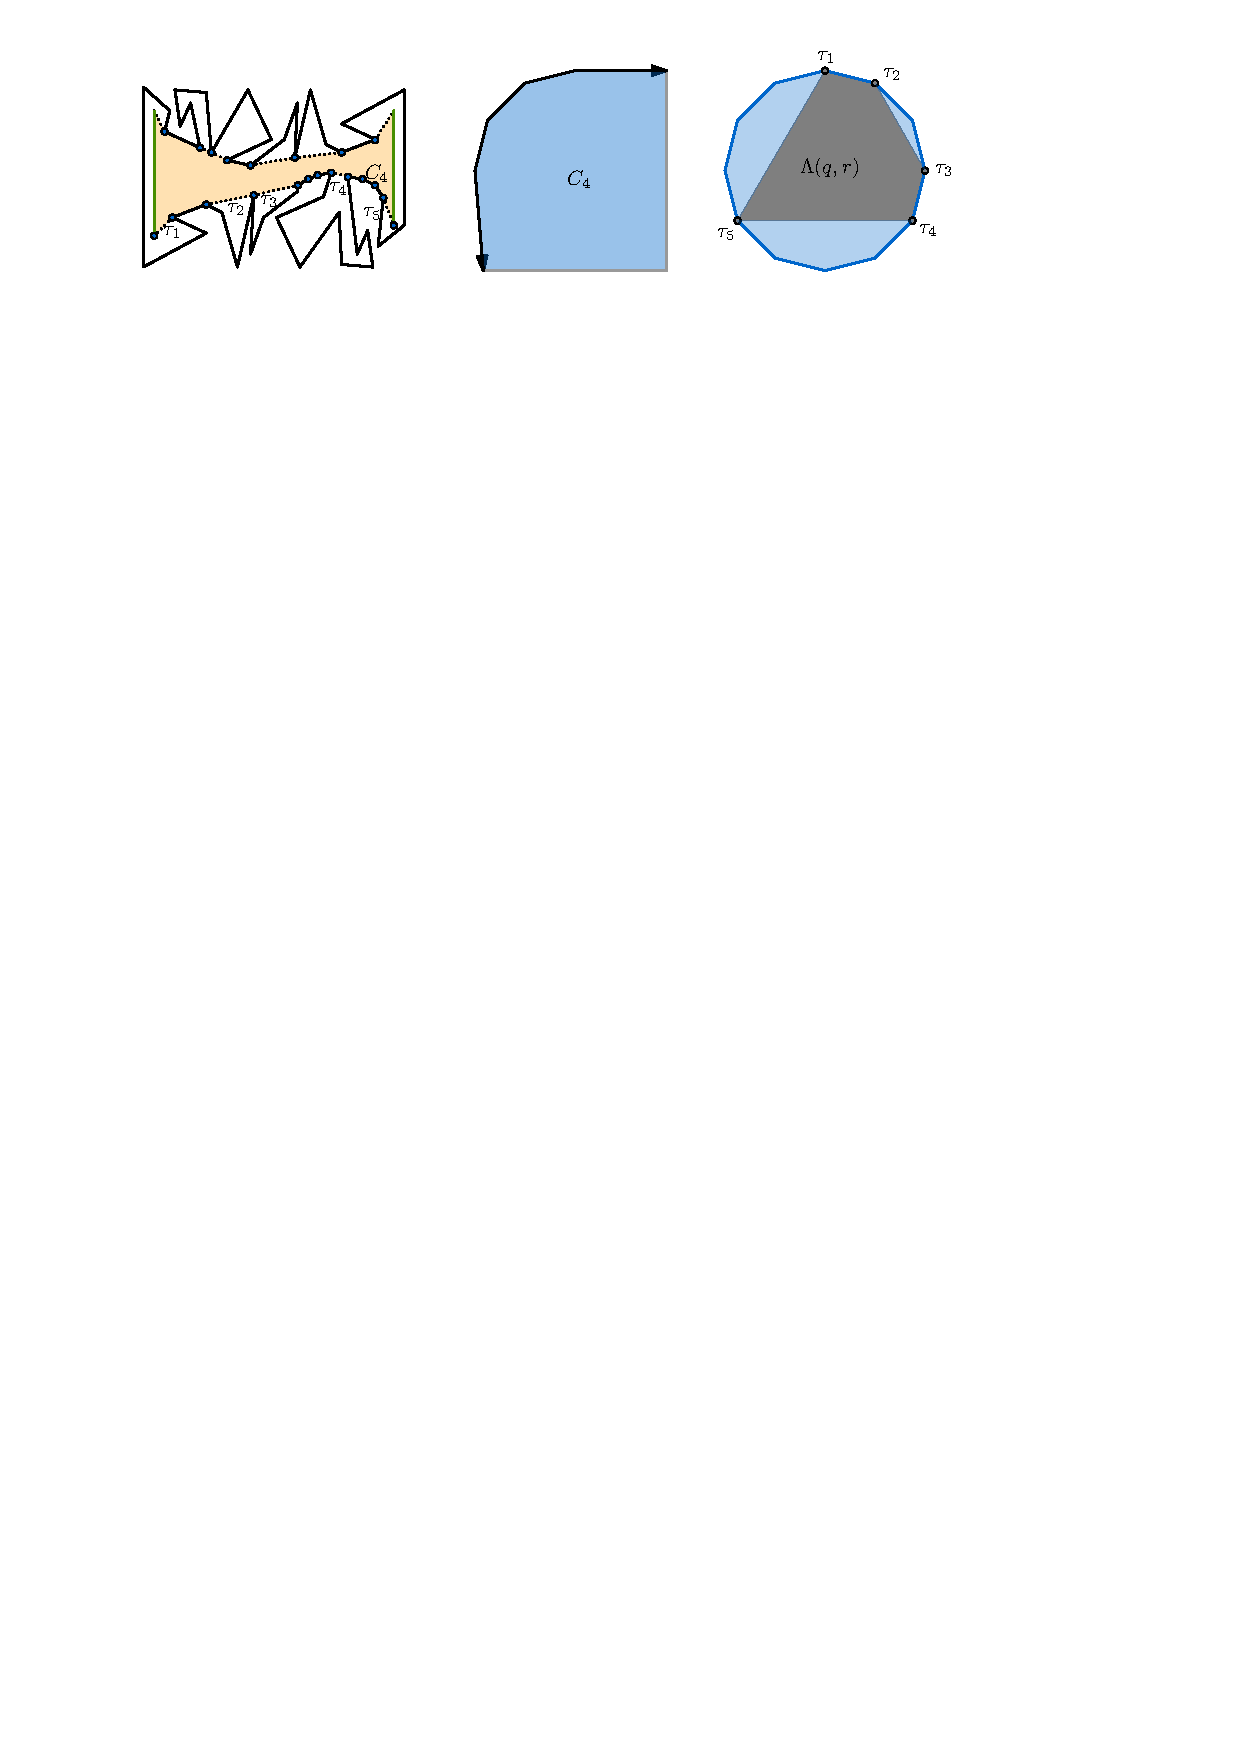
\includegraphics[]{../chain}
    \caption{(left) An hourglass between $q$ and $r$ in orange. The
      lower chain consists of five chains which coincide $P$ that are
      joined by outer tangents in dotted lines labelled $\tau_1 \ldots
      \tau_5$. (middle) An example of an area bound by the dualized
      chain $C_4$. (right) A simplified version of
      $\Lambda(q,r)$. Note that outer tangents could become vertices
      of $\Lambda(q,r)$. \frank{Fig left does not look like an
        hourglass to me; the chains are not semi-convex}}
    \label{fig:chain}
\end{figure}


\subparagraph{Querying the data structure.} When get a trajectory visibility
query with entities $q$ and $r$ we have to test if the curve $\gamma$ traced by
the point dual to the line through $q$ and $r$ intersects $\Lambda(q,r)$.
% (Observation~\ref{obs:visible})
By Observation~\ref{obs:obtain_L} the primal
representation $L(q,r)$ of $\Lambda(q,r)$ is an hourglass $H(q',r')$. We now
argue that: (i) we can find the subsegments $q'$ and $r'$ in $O(\log n)$ time,
(ii) that our data structure can report $O(\log^2 n)$ nodes from $T$ that
together represent an hourglass $H(q',r')$, and (iii) that we can then test if
$\gamma$ intersects $\Lambda(q,r)$ by using the associated data structures of
these reported nodes. This will result in $O(n^{\frac{3}{4}}\log^3 n)$ query
time.

\begin{lemma}
  \label{lemma:visibilityquery}
  Given our data structure, we can compute the subsegments $q' \subseteq q$ and $r' \subseteq r$ such that $L(q,r) = H(q',r')$ in $\O(\log n)$ time.
\end{lemma}

\begin{proof}
    By Observation~\ref{obs:obtain_L} the visibility glass $L(q,r)=H(q',r')$ for two sub-segments $q'$ and $r'$ which are bound by two edges which when extended form a bitangent of $H(q,r)$. We explained in the proof of Observation~\ref{obs:obtain_L} that the hourglass $H(q,r)$ had an upper and lower convex chain which may or may not share a vertex. The upper an can obtain the upper and lower chain both are a shortest path between endpoints of $q$ and $r$. We can obtain them using the data structure $\D$ from \cite{guibas1989optimal} as a balanced binary search tree and we can verify if they share a vertex using this tree. If that is the case then $L(q,r)$ is either empty or a single segment and we can verify this using an additional $\mathcal{O}(\log n)$ time. 
    
    If the upper and lower chain do not share a vertex then the segments $q'$ and $r'$ are bound by two bitangents. 
    Such a bitangent is the extension of an edge $(u,v)$ on the shortest path between two endpoints of $q$ and $r$. The edge $(u,v)$ is the unique edge on this path for which the path makes a clockwise turn at $u$ and a counterclockwise turn at $v$ or vice versa. Using $\D$ we can obtain any path as a balanced binary search tree. We perform a binary search on this tree to identify the edge $(u,v)$ whose endpoints have this unique clockwise ordering.
\end{proof}

We use Lemma~\ref{lemma:visibilityquery} to find the endpoints $q_1,q_2$ of
$q'$ and $r_1$, $r_2$ of $q'$ and $r'$, respectively. We can obtain the
shortest paths $\geod(r_1,q_1)$ and $\geod(r_2,q_2)$ bounding $L(q,r)=H(q',r')$
by concatenating $O(\log n)$ of the pre-stored hourglasses. To concatenate two
hourglasses we actually select two contiguous subchains in both hourglasses,
and compute two bridge edges connecting them. Such a contiguous subchain can be
represented by $O(\log n)$ nodes in the binary search trees representing the
hourglass boundary. It follows that $\geod(r_1,q_1)$ can be represented by
$O(\log^2 n)$ nodes; each representing a pre-stored subchain in the data
structure, together with $O(\log^2 n)$ line-segments (the bridge segments). We
now observe that the chains stored in the associated data structures of these
nodes, again together $O(\log^2 n)$ separate line segments $\Xi$, actually
represent the dual $\Lambda(q,r)$ of $L(q,r)$.

To check if the hyperbolic query segment $\gamma$ intersects $\Lambda(q,r)$ we
check if one of the endpoints of $Q$ lies in $\Lambda(q,r)$; in this case one
of the paths $\geod(r_1,q_1)$ or $\geod(r_2,q_2)$ is actually a single segment,
or if $\gamma$ intersects the boundary of $\Lambda(q,r)$. To this end, we query
each of these associated data structures. Since $\gamma$ has $k+1 = 5$ degrees of
freedom (Lemma~\ref{lemma:hyperbola}) this takes $O(n^{\frac{3}{4}}\log^3 n)$ time. We
test for intersection with the segments in $\Xi$ separately. We thus obtain the
following result.

\begin{theorem}
  \label{thm:data_structure_two_moving_monkeys_simple_polygon}
  Let $P$ be a simple polygon with $n$ vertices. In $O(n\log^5 n)$ time we can
  build a data structure of size $O(n\log^5 n)$ that can answer trajectory
  visibility queries in $O(n^{\frac{3}{4}}\log^3 n)$ time.
\end{theorem}

\section{Polygonal domains and trajectories intersecting edges}
\label{sec:variants}

We now consider the case where the trajectories can intersect a polygonal domain $P$. We include the special case where one trajectory is a stationary point.

\subsection{Two moving entities crossing edges in a polygonal domain}
\label{sub:Polygonal_Domain}

We investigate the two cases where (1) the entities can walk through
edges of $P$, and (2) where $P$ is a polygonal domain, simultaneously. Let $k$
be an unspecified constant. We prove that it is possible to transform the visibility query into a halfspace range query in $\mathbb{R}^k$ among $\mathcal{O}(n^3)$ points. Using cutting trees~\cite{chazelle1993cutting} we can preprocess the $\mathcal{O}(n^3)$ $k$-dimensional points representing $P$ using $\mathcal{O}(n^{3k})$ space and $\mathcal{O}(n^{3k})$ preprocessing time such that halfpace range queries (and thus our visibility query) can be answered in $\mathcal{O}(\log^k n)$ time.
%Our approach almost certainly does not generate an optimal solution with respect to its space requirement and query time. \frank{rephrase prev sentence} 
%However, it is a non-trivial proof that sub-linear query times are achievable. 
Details can be found in Appendix~\ref{app:Two_moving_entities_in_a_polygonal_domain}. 

Given a polygonal domain $P$ of $n$ vertices, we construct two near-identical data structures that test if there is line-of-sight between $q$ and $r$ with either positive or negative slope respectively. Let $t$ be a time where $q$ and $r$ are mutually visible and the line $g(t)$ through $q$ and $r$ has positive slope. The segment between $q$ and $r$ must be contained in a visibility glass $L(e_1, e_2)$ for two edges $e_1, e_2 \in P$. Consider the two points $p_1$ and $p_2$ which are the points of intersection between $g(t)$ and the edges $e_1$ and $e_2$. If $p_1$ lies below $p_2$, and $q$ lies below $r$, \patrick{I would phrase this as inequalities in $y$ instead of saying "below"} then, because $g(t)$ has a positive slope, we must have that $x_{p_1} \le x_{q} \le x_{r} \le x_{p_2}$.


This observation inspires the following approach: we consider for each pair of edges $e_1, e_2 \in P$, their dualized visibility glass $\Lambda(e_1,e_2)$, which we then triangulate. This results in a set $\mathcal{T}$ of $\mathcal{O}(n^3)$ triangles in the dual. Let $T \in \mathcal{T}$ be a triangle of $\Lambda(e_1, e_2)$, we lift $T$ to a two-dimensional surface in $\mathbb{R}^4$ (refer to Figure~\ref{fig:threedimensional} with the map $(a,b) \in T \rightarrow (a, b, x_{p_1}, x_{p_2})$ where $x_{p_1}$ is the $x$-coordinate of the intersection of the line $y = ax-b$ with the edge $e_1$. The two entities $q$ and $r$ have a unique associated degree-2 curve segment $\gamma$ which we also lift to $\mathbb{R}^4$ with the map $(a,b) \in \gamma \rightarrow (a,b, x_{q}, x_{r})$ where $x_q$ is the $x$-coordinate of entity $q$ at the time that realises the point $(a,b)$ on $\gamma$. It follows from this map and the observation above, that there is a time where $q$ and $r$ are mutually visible if and only if their $4$-dimensional curve intersects a 4-dimensional volume bound by a triangle $T \in \mathcal{T}$ and two orthogonal directions.

We transform $P$ into $\mathcal{O}(n^3)$ volumes in $\mathbb{R}^4$ which each have a constant-length description. Any query pair $q$ and $r$ gets mapped to a four-dimensional curve segment $\gamma'$ with constant description length. It follows that the predicate function specifying whether the segment $\gamma'$ intersects one of these volumes has constant description length and hence has a linearization into $k$ terms for some large constant $k$. There is a time where $q$ and $r$ are mutually visible if and only if there is an intersection.
We conclude:

\begin{theorem}
 \label{thm:polygonal_moving}
  Let $P$ be a polygonal domain with $n$ vertices, and let $k$ be some sufficiently large constant. In $O(n^{3k})$ time we
  can build a data structure of size $O(n^{3k})$ that can answer
  trajectory visibility queries in $\mathcal{O}(\log^k n)$ time.
\end{theorem}

 
 
 \subsection{A data structure for queries with one moving entity}
 \label{sec:pointline}
 
 Finally, we consider the special case where $q$ is a point and $r$ is a segment.
 Clearly, our results for the more general scenario apply to this case as well. However, we can achieve better results using a different approach. Next, we briefly describe the main ideas. A more thorough description can be found in Appendix~\ref{app:pointline}.
 
 When $P$ is a simple polygon and $r$ is contained in $P$ we build the shortest path data structure from Guibas and Hershberger~\cite{guibas1989optimal} on the simple polygon $P$. At query time, we use this data structure to obtain the two shortest paths between the endpoints of $r$ and the entity $q$. We show that we can inspect these paths in constant time each, to detect if there is a time where $q$ and $r$ are mutually visible.
 
\begin{theorem}
\label{thm:one_dead_one_alive}
  Let $P$ be a simple polygon with $n$ vertices. In $\O(n)$ time we
  can build a data structure of size $\O(n)$ with which we can test if
  there is a time at which a stationary entity can see a linearly
  moving entity in $\O(\log n)$ time.
  % We can preprocess a simple polygon $P$ in $\Theta(n)$ space and
  % $\Theta(n)$ time. Such that for any query point $q$ and segment
  % trajectory $r$ which is contained in $P$, we can determine if there
  % is a point on $r$ that is visible from $q$ in $\Theta(\log n)$ time.
\end{theorem}
 
 When $P$ is a simple polygon but the trajectory of $r$ may intersect edges
of $P$ is significantly more difficult. 
Let $V_q$ denote the \emph{visibility polygon} of point $q$: the set
of all points visible from $q$. There is a time at which $q$ can see
$r$ if and only if the trajectory of $r$ intersects (the boundary of)
$V_q$. We build a data structure to find such a point (if one
exists). To this end we extend a result of 
Aronov~\etal~\cite{aronov2002visibility}. They developed an $\O(n^2)$ size
data structure that can be built in $\O(n^2\log n)$ time and can report the
visibility polygon of an arbitrary query point $q \in P$ in $\O(\log^2 n)$
time. The visibility polygon $V_q$ is returned in its combinatorial
representation, that is, as a (pointer to a) balanced binary search tree,
storing the vertices of $V_q$ in order along the boundary. This combinatorial representation does not explicitly store the
locations of all vertices of $V_q$. Instead, a vertex $v$ of $V_q$ may be
represented by a pair $(e,w)$, indicating that $v$ is the intersection point of polygon edge $e$ and the line through vertex $w \in P$ and the query point
$q$. Computing the explicit location of all vertices of $V_q$ thus takes
$\O(|V_q|)$ time by traversing the tree.

We extend the above results using semi-algebraic range searching so that we can efficiently test if a line segment intersects $V_q$ \emph{without} spending the $\O(|V_q|)$ time to compute the explicit locations.
Suppose that the entity $r$ cuts off a vertex $v$ of $V_q$ represented by a pair $(e,w)$ then the vertex $v$ and the entity $q$ must lie on either side of the line through $r$. This observation leads to a predicate function $F( (e,w), (q,r))$ that outputs a negative real number if and only if the entity $q$ and the vertex $v$ lie on either side of $r$. We make several non-trivial observations about $V_q$ and the Aronov \etal data structure that allows us to express this predicate function with as few variables as possible. The result is that we can transform the question of whether $r$ intersects $|V_q|$ into a halfspace emptyness query in $\mathbb{R}^8$. We therefore obtain the following result.

\begin{theorem}
  \label{thm:one_dead_one_ghost}
  Let $P$ be a simple polygon with $n$ vertices. In $O(n^2\log^3 n)$ time We
  can build a data structure of size $O(n^2\log^3 n)$ that can answer
  trajectory visibility queries between a static entity $q$ and a linearly
  moving entity $r$ that may cross $P$ in $O(n^{\frac{3}{4}+\eps})$ time.
\end{theorem}

When $P$ is a polygonal domain and $r$ may intersect edges of $P$ we essentially use the same ideas as in the previous case. In this case, the base data structure to obtain the visibility polygon $V_q$ uses $O(n^4)$ rather than $O(n^2)$ space.

\begin{theorem} 
\label{thm:full_domain}
  Let $P$ be a polygonal domain with $n$ vertices. In $O(n^4\log^3 n)$ time We
  can build a data structure of size $O(n^4\log^3 n)$ that can answer
  trajectory visibility queries between a static entity $q$ and a linearly
  moving entity $r$ that may cross $P$ in $O(n^{\frac{3}{4}+\eps})$ time.    
\end{theorem}
 
 
 
 
 
 
 
 
 
 
 
 
 

% \section {Conclusions}
% \label {sec:conclusions}

% Future work:

% * We want to improve our results, or find lower bounds (the obvious one)

% * Now that we better understand the algorithmic complexity of the question whether two moving entities can see each other at all, we may also consider more complex questions, such as
% - when do they see each other
% - how often do they see (start seeing) each other
% - how long do they see each other (in total or consecutively)

% * We could say something about the uncertain trajectories application

\newpage
\bibliographystyle{abbrv}
\bibliography{bib}

\newpage
\appendix

\section{Transforming two entites into an algebraic curve.}
\label{app:hyperbola}


Throughout this paper, we study the line-of-sight between two entities that each move along a linear trajectory (possibly at different but constant speeds) during the time $t \in [0,1]$. Consider the line $g(t)$ through the two entities at time $t$. We can dualize $g(t)$ to a point using classical point-line dualization. In Section~\ref{sec:prelims} we claim that the continuous dualization of the line through the two entities traces a degree-2 curve segment denoted by $\gamma$ in the dual. Here we show why this is the case:

\begin{repeatlemma}{lemma:hyperbola}
  The segment $\gamma$ is a segment of a hyperbolic curve with $5$ degrees of freedom.
\end{repeatlemma}

\begin{proof}%[Proof of Lemma~\ref{lemma:hyperbola}]
For algebraic convenience we say that entity $q$ walks from $(a_1, a_2)$ to $(a_1 + a_3, a_2 + a_4)$ and that entity $r$ walks from $(a_5, a_6)$ to $(a_5 + a_7, a_6 + a_8)$. Note that the speed of entity $q$ is $\lVert (a_3, a_4) \rVert$ and that the speed of entity $r$ is $\lVert (a_7, a_8) \rVert$. We can parametrize the position of entity $q$ and $r$ on the time $t \in [0,1]$ as follows:

\begin{equation}
    \label{eq:line}
     q(t) = \left( \begin{array}{c}
         x_{q(t)}  \\
         y_{q(t)} 
    \end{array}  \right) = 
    \left( \begin{array}{c}
         a_1 + a_3 t \\
         a_2 + a_4 t
    \end{array}  \right)  \quad
      r(t) = \left( \begin{array}{c}
         x_{r(t)}  \\
         y_{r(t)} 
    \end{array}  \right) = 
    \left( \begin{array}{c}
         a_5 + a_7 t \\
         a_6 + a_8 t
    \end{array}  \right) 
\end{equation}


At all times, the line $g(t)$ is the line through the points $q(t)$ and $r(t)$. We say that at all times, $g(t)$ has slope and offset $(\alpha(t), \beta(t))$. The parametrisation of $g(t)$ then becomes:

\begin{equation}
\label{eq:curve}
   g(t) = \left( \begin{array}{c}
         \alpha(t)  \\
         \beta(t) 
    \end{array}  \right) = 
    \left( \begin{array}{c}
         \frac{y_{r(t)} - y_{q(t)}}{x_{r(t)} - x_{q(t)}}  \\
         \alpha(t)\cdot x_{q(t)} - y_{q(t)}
    \end{array}  \right) =
    \left( \begin{array}{c}
         \frac{ a_6 - a_2 + (a_8 - a_4) t}
      { a_5 - a_1  + (a_7 - a_3) t }  \\
         \alpha(t) (a_1 - a_3 t) - a_2 - a_4 t 
    \end{array}  \right)
  \end{equation}
  
  If the time $t$ lies between $0$ and $1$, this parametric equation traces our curve segment $\gamma$ and if we take $t$ over all of $\mathbb{R}$, the parametric equation traces a full curve which we denote by $\Gamma$. To show the degree of the curve $\Gamma$ we rewrite the parametrized curve to a canonical form that drops the dependence on $t$. First we take the formula for the $\beta$-coordinate and isolate $t$:
  
  \[
     t = \frac{\alpha(t) a_1 - a_2  - \beta(t)}{\alpha(t) a_3 + a_4}
  \]
We then take the formula for the $\alpha$-coordinate and remove the fraction by multiplying both sides with $ ((a_5 - a_1)  + (a_7 - a_3) t)$:

\[ 
\alpha(t)(a_5 - a_1)  + \alpha(t)(a_7 - a_3) t = (a_6 - a_2) + (a_8 - a_4) t
\]

We substitute the value for $t$ into this equation, and remove the fraction by multiplying both sides with $(\alpha(t) a_3 + a_4)$:

\begin{align*}
\alpha(t)(\alpha(t) a_3 + a_4)(a_5 - a_1)  + \alpha(t)(a_7 - a_3) (\alpha(t) a_1 - a_2  - \beta(t)) = \\
(a_6 - a_2)(\alpha(t) a_3 + a_4) + (a_8 - a_4) (\alpha(t) a_1 - a_2  - \beta(t)) \Rightarrow \\
\alpha(t)^2a_3(a_5 - a_1) + \alpha(t)a_4(a_5 - a_1)  + \alpha(t)^2a_1(a_7 - a_3)
- \alpha(t)a_2(a_7 - a_3)  - \alpha(t)\beta(t)(a_7 - a_3) = \\
\alpha(t) a_3(a_6 - a_2) + a_4(a_6 - a_2) + \alpha(t)a_1(a_8 - a_4) - a_2 (a_8 - a_4) - \beta(t)(a_8 - a_4) 
\end{align*}

Lastly we linearize this equation by separating polynomials based on $\alpha(t)$ and $\beta(t)$ from polynomials based on $a_1 \ldots a_8$.

\begin{align}
\label{eq:hyperbola}
    0= [\alpha(t)^2](a_5 a_3 -2 a_1 a_3 + a_1 a_7)+ \\
    [\alpha(t)](a_4 a_5 - a_3 a_6 + a_2 (2 a_3 - a_7) - a_1 a_8) + \\
    [\alpha(t)\beta(t)](-(a_7 - a_3)) + [\beta(t)](-(a_8 - a_4)) + [1](a_4(a_6 - a_2)- a_2 (a_8 - a_4))
\end{align}
\end{proof}


\section{Semi-algebraic range searching}
\label{appx:rangesearch}

%\subsection{An introduction to semi-algebraic range searching and some examples.}
\label{appx:introduction}

Throughout this paper we make extensive use of the semi-algebraic (or linearization) techniques from Agarwal \etal \cite{agarwal2013range}. 
%This appendix section contains an extended introduction to these techniques.
We describe the technique in detail for completeness.

Let $X$ be a set of $n$ geometric objects in $\mathbb{R}^d$, where each object is parametrized by a vector $\vec{x}$. If $X$ is a set of points, then the most natural parametrization is a vector of its coordinates. But $X$ could be a more complicated algebraic object such as a line, in that case the most natural parametrization is a two-dimensional vector containing its slope and offset.

We denote by $\Gamma$ be a family of geometric regions (called semi-algebraic ranges) in $\mathbb{R}^d$ where each region $G \in \Gamma$ is bound by an algebraic curve $\gamma$ which is parametrized by a vector $\vec{a}$. Two examples of such a family is the set of all disks and the set of all disks of radius 1. An arbitrary disk can be represented as a vector in many ways: three non-colinear points define a unique circle so one could represent a circle as a six-dimensional vector which specifies the coordinates of these points. However the larger the representation vector, the more complicated the linearization process becomes. The most efficient representation of a circle is by a three-dimensional vector specifying its center and radius. The family of disks of radius 1 has fewer degrees of freedom than the family of all disks, and thus their representation can be more efficiently represented (e.g. as a 2-dimensional vector specifying only its center).

Given $X$ and $\Gamma$, we are interested in preprocessing $X$ such that for any range $G \in \Gamma$, we can report which objects of $X$ intersect $G$. To accomplish this, we first want to derive what we have dubbed a \emph{predicate function} $F(\vec{x}, \vec{a}) \le 0$. The predicate function $F$ takes any instance of $X$ (parametrized by $\vec{x}$) and any instance of $\Gamma$ (parametrized by $\vec{a}$) and outputs a real number. The object intersects the range if and only if the output value is lesser-or-equal to zero. At this point we present an example: let $X$ be a set of two-dimensional points parametrized by $\vec{x} = (x_1, x_2)$ and $\Gamma$ be the set of arbitrary disks, each parametrized by $\vec{a} = (a_1, a_2, r)$. The disk parametrized by $\vec{a}$ has center $(a_1, a_2)$ and radius $r$. Any point $(x_1, x_2)$ is contained in this disk if and only if $F(\vec{x}, \vec{a}) = (a_1 - x_1)^2 + (a_2 - x_2)^2 - r^2 \le 0$ and thus we have found our predicate function.

The predicate function $F(\vec{x}, \vec{a})$ could be seen as a map from the parameter space of our intersection problem to the boolean space $\{0,1\}$ and thus $F$ partitions our parameter space into areas where the answer is \emph{yes} or areas where the answer is \emph{no}. The idea behind semi-algebraic range searching is that we search for an intersection in this parameter space, as opposed to searching in the space where our problem lives. However, the border of these areas do not have to be particularly nice. In our example. each of the \emph{yes} areas is bound by a quadratic surface. This is where \emph{linearization} comes in. We transform the parameter space through a polynomial map into a $k$-dimensional space where the boundary of the \emph{yes} spaces become linear-complexity surfaces. From there on, we can solve our problem using halfspace range searching. Specifically, we rewrite the function $F(\vec{x}, \vec{a})$ to the form: $F(\vec{x}, \vec{a}) =  g_0(\vec{a}) + \sum_{i=1}^k g_i(\vec{a})f_i(\vec{x})$ where $f_i$ and $g_i$ are polynomials dependent only on $\vec{x}$ and $\vec{a}$ respectively. In our example we had: $F(\vec{x}, \vec{a}) = (a_1 - x_1)^2 + (a_2 - x_2)^2 - r^2 \le 0$. To linearize this function we need to first expand the squares: $F(\vec{a}, vec{x}) = a_1^2 - 2 a_1 x_1 + x_1^2 + a_2^2 - 2 a_2 x_2 + x_2^2 - r^2$. This immediately gives a straight-forward linearization of seven terms. However, we can reduce the number of terms by grouping variables and writing: $F(\vec{x}, \vec{a} = [a_1^2 + a_2^2 - r^2] + [-2 a_1](x_1) + [-2 a_2](x_2) + [1](x_1^2 + x_2^2)$ and obtain a linearization where: $(g_0, g_1, g_2, g_3) = (a_1^2 + a_2^2 - r^2, -2a_1, -2a_2, 1)$ and $(f_1, f_2, f_3) = (x_1, x_2, x_1^2 + x_2^2)$. We get the term $g_0$ (which is not attached to any polynomial dependent on $x$) ``for free'' and this thus becomes a three-dimensional linearization.

Agarwal \etal prove that you can map any $d$-dimensional point $\vec{x}$ to the $k$-dimensional point $f(\vec{x}) = (f_1(\vec{x}), f_2(\vec{x}), \dots f_k(\vec{x}))$, and any query range to the $k$-dimensional halfspace $G(\vec{a}) = \left\{ \vec{y} \in \mathbb{R}^k \mid g_0(\vec{a})  + \sum_i^k g_i(\vec{a})y_i  \le 0 \right\}$ and that $\vec{x}$ intersects $G$ if and only if $f(\vec{x})$ is contained in $G(\vec{a})$. 
Consider our example. The map $f$ that we found, is the well-known parabeloid projection: We map all the two-dimensional points onto a three-dimensional parabeloid and they are contained in a circle $G \in G$ if and only if the points lie within a halfplane cutting the parabeloid.  Refer to Figure~\ref{fig:algebraic} for an even shorter example.


\begin{figure}[tb]
    \centering
    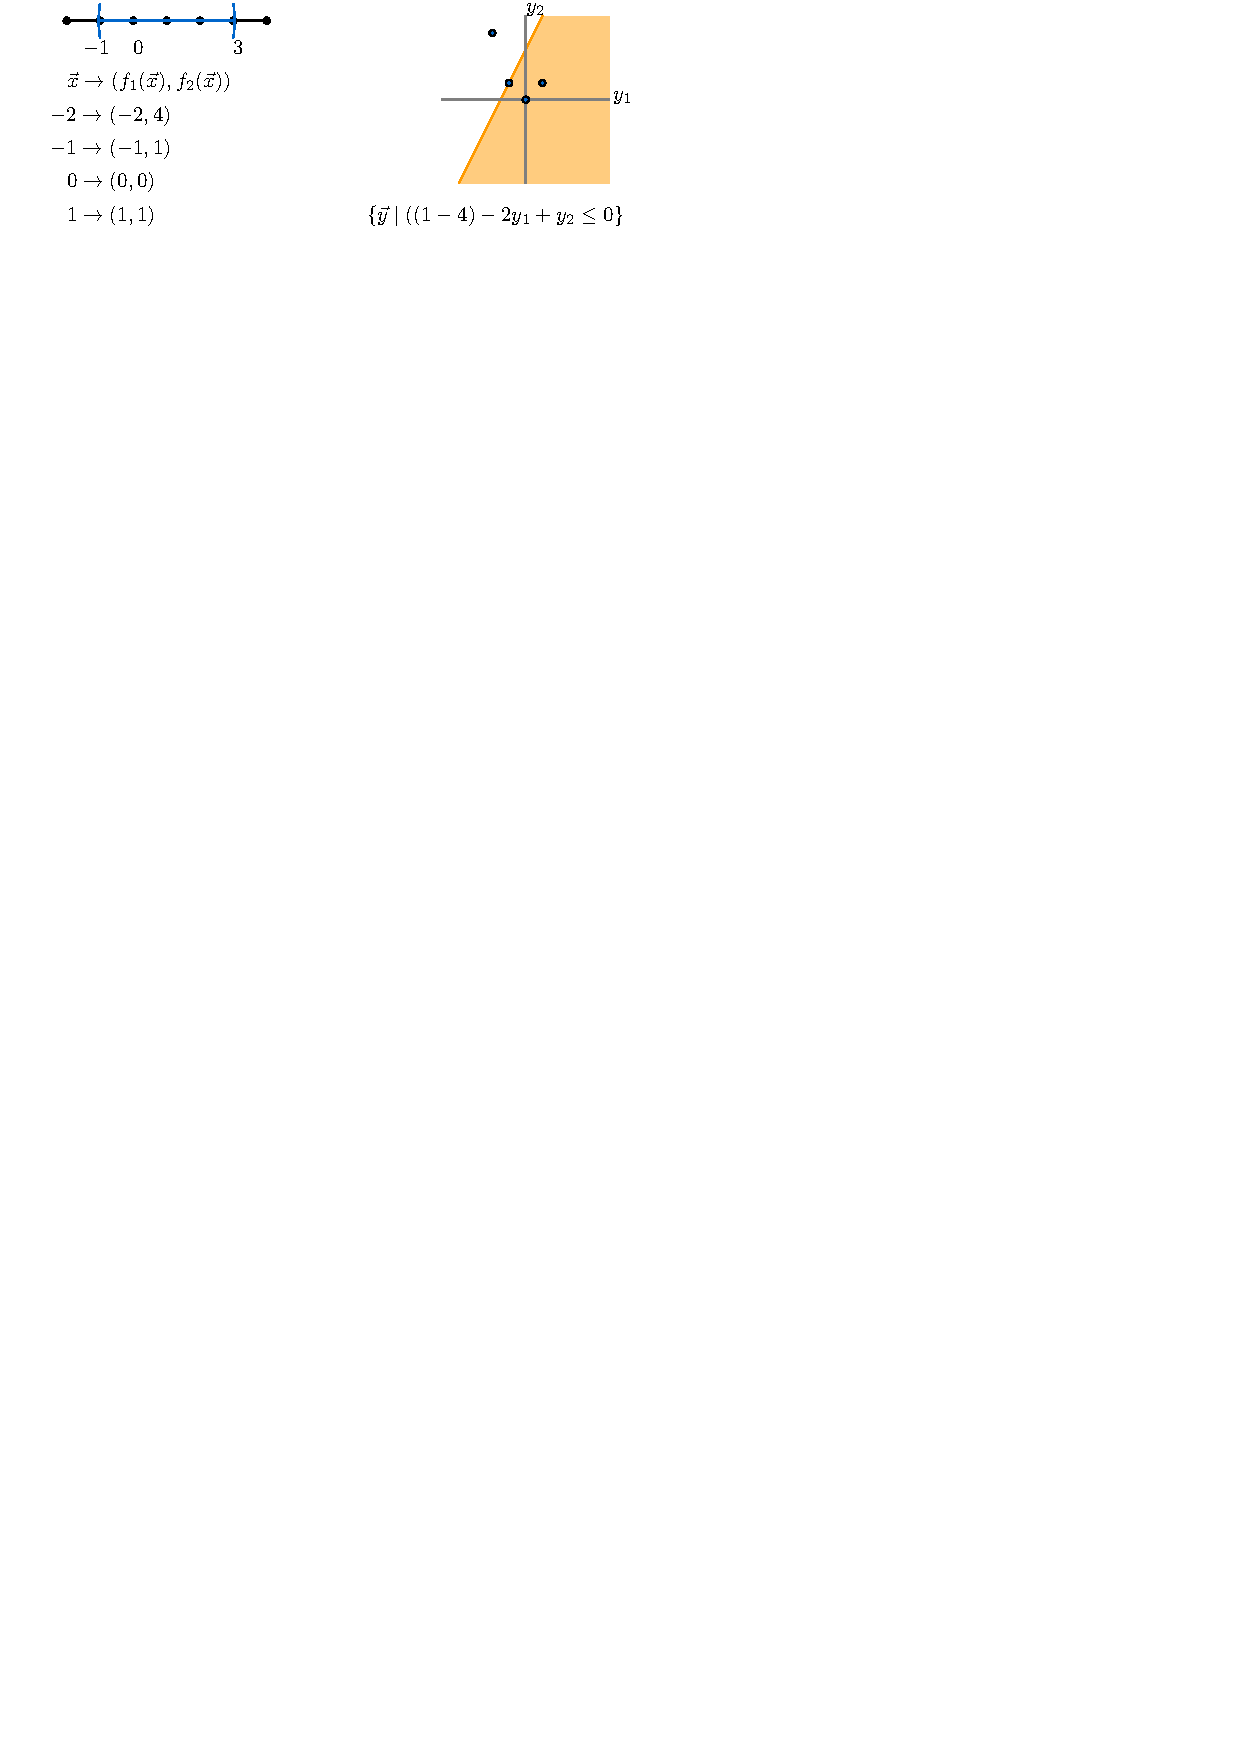
\includegraphics{../algebraic}
    \caption{Consider the family $\Gamma$ of 1-dimensional unit disks. We can parametric their border by supplying a 1-dimensional center point and a radius $\vec{a}=(a_1, a_2)$. Any 1-dimensional point $\vec{x} = (x_1)$ is contained in a disk $G \in \Gamma$ if and only if $(a_1 - x_1)^2 - a_2^2 \le 0 Rightarrow [a_1^2 - a_2^2] + [-2a_1](x_1) + (x_1^2) \le 0$. If we linearize this predicate function, we get that $(g_0, g_1, g_2) = (a_1^2 - a_2^2, -2a_1, 1)$  and $(f_1, f_2) = (x_1, x_1^2)$. It follows that any intersection query between a disk $G$ and a set of points $X$ can be answered using a halfspace emptyness query. In the figure we show an example for the points $(-2, -1, 0, 1)$ and the disk $G$ with center 1 and radius 2. }
    \label{fig:algebraic}
\end{figure}

\subsection{Intersecting line segments with a quadratic curve segment}
\label{sub:intersecting_line_segments_with_a_quadratic__curve_segment}

Let $E$ be a set of $n$ line segments. We describe how to preprocess
$E$ such that for an arbitrary degree-2 curve segment $\gamma$ we can
test if $\gamma$ intersects an edge of $E$ in sublinear. More
specifically, we establish the following result:

\begin{lemma}
  \label{lemma:15000}
  Let $E$ be a set of $n$ line segments. In $\O(n\log n)$ time, we can
  construct a linear size data structure that can test if an arbitrary
  degree-2 query curve segment $\gamma$ intersects a segment in $E$
  (and if so report it) in $O(n^{1-\frac{1}{15 000}})$ time.
  % structure of linear size, 
  % We can preprocess a set $E$ of line segments using $\mathcal{O}(n)$
  % space and $\mathcal{O}(n)$ construction time, such that an
  % intersection (if any exists) between an arbitrary degree-2 curve
  % segment $\gamma$ and an edge in $E$ can be found in
  % $\mathcal{O}(n^{1-\frac{1}{15000}})$ time.
\end{lemma}


% prove that we can preprocess \emph{any} set of edges $E$, such that we can test for an intersection between an arbitrary degree-2 curve segment $\gamma$ and an edge in $E$ in sub-linear time.  This means that the set of edges $E$ does not have to be connected, convex or even non-intersecting. We first provide a proof outline and then the formal proof.

% In Section~\ref{sec:intersectionsearch} we describe how to preproces a convex simple polygon $P_E$ formed by a set of edges $E$ such that for any segment $\gamma$ of an arbitrary degree-2 curve $\Gamma$, we can test if $P_E$ is intersected by $\gamma$ in sub-linear time. In the section we explain that we first make many geometric observations about $P_E$ and that we only implore semi-algebraic range searching in the last step. We note that it is possible to immediately implore semi-algebraic range searching but that this leads to a less efficient solution. Although this solution brings worse bounds, the solution is more general: We specifically prove that we can preprocess \emph{any} set of edges $E$, such that we can test for an intersection between an arbitrary degree-2 curve segment $\gamma$ and an edge in $E$ in sub-linear time.  This means that the set of edges $E$ does not have to be connected, convex or even non-intersecting. We first provide a proof outline and then the formal proof.

\subparagraph*{Proof outline.}
As an object set we are given a set $E$ of arbitrary edges with no restrictions. We say that an edge $e \in E$ goes from the point $(x_1, x_2)$ to the point $(x_1 + x_3, x_2 + x_4)$ and thus parametrize each edge as a vector $\vec{x} = (x_1, x_2, x_3, x_4)$. As a query family, we are given the family $\Gamma$ of degree-2 curve segments which are parametrized according to equation~\ref{eq:hyperbola} with a parametrization vector $\vec{a} = (a_1 \ldots a_8)$. The goal is to design a predicate function $F(\vec{x}, \vec{a})$ that takes any pair of edge and query curve and that outputs a number. The query curve should intersect the edge if and only if the output number is less than zero. Specifically, we design \emph{four} predicate functions $F_1, F_2, F_3, F_4$ and the query curve intersects the edge if and only if all four predicates output a number less than zero. This can be checked by using four consecutive halfspace-range queries.

We detect for an intersection between an arbitrary $\gamma$ in three steps:
\begin{enumerate}
    \item First we rotate and shear the plane, using the parameter vector $\vec{x}$, such that the edge $e$ starts at $(0,0)$ and ends at $(0, \lVert (x_3, x_4) \rVert$. We now know, that $\gamma$ can only intersect the edge at a point where its $x$-coordinate is $0$. 
    \item We algebraically compute the at most 2 times $t, t'$, where the $x$-coordinate of the full curve supporting $\gamma$ is zero and we check if $0 \le t, t' \le 1$. This gives the first two predicate functions $F_1, F_2$. If this is not the case for either $t$, then we know that $\gamma$ cannot intersect the edge $e$.
    \item As a third step, we fill in the times $t, t'$ where the first coordinate of the curve supporting $\gamma$ is zero and we check if the second coordinate lies between $0$ and $ \lVert (x_3, x_4) \rVert$. If this is not the case, then the curve goes over or under the line segment. This gives the last two predicate functions $F_3$ and $F_4$.
\end{enumerate}

Having computed the predicates $F_1, F_2, F_3, F_4$, we need to linearize them. And we linearize them using approximately 15000 terms. We want to briefly mention why this number is so high. In its general form, the predicate has twelve unrestricted variables $x_1 \ldots x_4$ and $a_1 \ldots a_8$. One can imagine, that twelve unrestricted variables leads to a formula with at least twelve linear terms.

At step 2, we compute the time $t$ for which the first coordinate of the degree-2 curve is zero. To do this, we need to make use of the quadratic equation and that will give us a square root containing both variables from $\vec{x}$ and $\vec{a}$. If we want to linearize, we need to get rid of the square root. That means squaring both sides and expanding the resulting equation which implies quadratically many more linear terms. At step 3, a similar thing happens and we again have to resolve a square root. We started with $12$ terms and we squared twice, which would naively give us $20.000$ terms.



\paragraph*{A proof of a more restricted case that linearizes to $\mathbb{R}^3$.}
We first want to show that the approach that we suggested above can be an efficient way to compute the intersection between algebraic objects. % If you are only interested in the formal proof of Lemma~\ref{lemma:15000}, please skip ahead to the next subsection.

Consider the set $E$ of arbitrary line segments, and the family of regions $\Gamma'$ where each range $G \in \Gamma'$ is a \emph{line segment} (hence, a more restricted degree-2 curve). Agarwal notes \cite{agarwal2004range} that the intersection between an edge $e \in E$ and segment $G \in \Gamma$ can be written as a predicate with three linear terms. Most likely, Agarwal uses the cross product between the segments for this linearization and this approach does not generalize to curves. We show that with our approach, you also get a linearization of three terms. 

We assume that each edge $e$ in $E$ is from the point $(x_1, x_2)$ to $(x_1 + x_3, x_2 + x_4)$ and that each query $G$ in $\Gamma'$ is a segment from the point $(a_1, a_2)$ to $(a_1 + a_3, a_2 + a_4)$. The first step is to translate and shear the plane.
First we translate the plane with the vector $-(x_1, x_2)$ such that $e$ starts at the origin. Then we shear the plane with the following map: $(x,y) \rightarrow (x - \frac{x_3}{x_4}y, y)$ such that $e$ points upwards. 
If we apply our translation and shearing, we get a new segment $G'(t)$ whose parametrization on $t$ is:

\begin{align*}
    &G'(t) = R(x_3, x_4) \cdot (G(t) - (x_1, x_2)) =  
    \left( \begin{array}{c}
         x  \\
         y 
    \end{array} \right) =
    \left( \begin{array}{c}
         (a_1 - x_1 + t a_3) - \frac{x_3}{x_4}(a_2 - x_2 + t a_4 )  \\
         a_2 - x_2 + t a_4 
    \end{array} \right)
\end{align*}
The first thing that we do, is that we compute the time $t^*$ for which the $x$-coordinate of this transformed query segment $G'(t)$ is zero.

\begin{align*}
    x = 0 \Rightarrow \\
    0 = (a_1 - x_1 + t a_3) - \frac{x_3}{x_4}(a_2 - x_2 + t a_4 )   \Rightarrow \\
    - t ( a_3 -  \frac{x_3}{x_4} a_4) = a_1 - x_1 - \frac{x_3}{x_4} (a_2 - x_2) \Rightarrow \\
    %
    t = \frac{   a_1 - x_1 - \frac{x_3}{x_4} (a_2 - x_2)}{ - a_3 + \frac{x_3}{x_4}a_4}
\end{align*}

The first predicate verifies whether or not $t^*$ is greater or equal than $0$:

\begin{align*}
    0 \le t \Rightarrow \\
   0 \le F_1(\vec{x}, \vec{a}) = a_1 - x_1 - \frac{x_3}{x_4} (a_2 - x_2)  \\
    %
    0 = (a_1) + (1)[\frac{x_3}{x_4}x_2 - x_1] + (a_2) [ - \frac{x_3}{x_4} ] \\
    \textnormal{Hence we have a predicate } F_1 \textnormal{ Where }\\
    %
    A_0(\vec{a}) = a_1, \quad A_1(\vec{a}) = 1,\quad A_2(\vec{a}) = a_2 \\
    %
    f_1(\vec{x}) = \frac{x_3}{x_4}x_2 - x_1 \quad f_2(\vec{x}) = - \frac{x_3}{x_4}
\end{align*}

The second predicate verifies whether or not $t^*$ is lesser or equal to $1$:

\begin{align*}
    &t \le 1 \Rightarrow \\
    & a_1 - x_1 - \frac{x_3}{x_4} (a_2 - x_2) \le  - a_3 + \frac{x_3}{x_4}a_4 \\
    & a_1 - x_1 - \frac{x_3}{x_4} (a_2 - x_2) + a_3 - \frac{x_3}{x_4}a_4 \le 0 \\
    %
    &0 \ge F_2(\vec{x}, \vec{a}) = (a_1 + a_3) + (1)[\frac{x_3}{x_4}x_2- x_1] + (a_2 + a_4) [ - \frac{x_3}{x_4} ] \\
    %
    \textnormal{Hence we have a predicate } F_2 \textnormal{ Where } \\
    %
    &A_0(\vec{a}) = a_1 + a_3, \quad A_1(\vec{a}) = 1,\quad A_2(\vec{a}) = a_2 + a_4 \\
    %
    &f_1(\vec{x}) = \frac{x_3}{x_4}x_2- x_1,\quad f_2(\vec{x}) = - \frac{x_3}{x_4}
\end{align*}

The third predicate, verifies whether not the $y$ value of $G'(t^*)$ lies below $\sqrt{x_3^2 + x_4^2}$:

\begin{align*}
    y_{G'(t^*)} = a_2 - x_2 + t^* a_4   \le \sqrt{x_3^2 + x_4^2} \Rightarrow \\
    %
    a_2 - x_2 + a_4 \frac{   a_1 - x_1 - \frac{x_3}{x_4} (a_2 - x_2)}{ - a_3 + \frac{x_3}{x_4}a_4} \le \sqrt{x_3^2 + x_4^2} 
\end{align*}

We multiply both sides by $- a_3 + \frac{x_3}{x_4}a_4$ and obtain:


\begin{align*}
    (- a_2 a_3) +  (a_2 a_4) \left[\frac{x_3}{x_4}\right] +  (a_3)[x_2] + (a_4)[ - \frac{x_3}{x_4}x_2] + (a_4 a_1) + (a_4)[ \frac{x_3}{x_4}x_2 - x_1] - (a_2a_4)\left[\frac{x_3}{x_4}\right]
        \le \\
    (- a_3)[ \sqrt{x_3^2 + x_4^2} ] + (a_4) [\frac{x_3}{x_4} \sqrt{x_3^2 + x_4^2}] \Rightarrow \\
    (a_1 a_4 - a_2 a_3) + (a_3)[x_2 - \sqrt{x_3^2 + x_4^2}] + (a_4)[ - \frac{x_3}{x_4}( x_2 + \sqrt{x_3^2 + x_4^2}) -x_1 ] \le 0 \\
        %
    \textnormal{Hence we have a predicate } F_2 \textnormal{ Where } \\
    %
    A_0(\vec{a}) = a_1 a_4 - a_2 a_3, \quad A_1(\vec{a}) = a_3, \quad A_2(\vec{a}) = a_4 \\
    %
   f_1(\vec{x}) = \frac{x_3}{x_4}, \quad f_2(\vec{x}) =  x_2 - \sqrt{x_3^2 + x_4^2}, \quad f_3(\vec{x}) = - \frac{x_3}{x_4}( x_2 + \sqrt{x_3^2 + x_4^2}) -x_1
\end{align*}

The predicate $F_4$ checks if the $y$-value is above $0$. It is the same predicate as $F_3$ with the terms dependent on $\sqrt{x_3^2 + x_4^2}$. It follows that we can verify if a query segment intersects an edge in $E$ using four predicates which each have at most 3 terms. 

\paragraph*{Poof of Lemma~\ref{lemma:15000}.}

Lastly, we provide the complete proof for Lemma~\ref{lemma:15000}. Denote by $\gamma$ any segment parametrized by a vector $\vec{a}$ according to equation~\ref{eq:hyperbola}. The algebraic formulations will get very long, so for succinctness we denote $A_i = a_i - a_{i-4}$. The formulation for $\gamma$ dependent on $t$ now becomes:

\begin{equation}
  \gamma(t) = \left( \begin{array}{c}
         x  \\
         y 
    \end{array}  \right) =  
        \left( \begin{array}{c}
         \frac{ A_6 + A_8 t}
      { A_5  + A_7 t } \\
         a(t)(a_1 +  a_3 t) - a_2 -  a_4 t 
    \end{array}  \right)
\end{equation}

Removing brackets and applying the translation gives:

  \begin{equation*}
   \gamma(t)_T = \left( \begin{array}{c}
         x  \\
         y 
    \end{array}  \right) = 
    \left( \begin{array}{c}
         \frac{ A_6 + A_8 t}
      { A_5  + A_7 t } - x_1 \\
         \frac{ A_6 a_1 + A_8 a_1 t + A_6 a_3 t + A_8 a_3 t^2 }{A_5 + A_7t} - a_2 - a_4 t - x_2
    \end{array}  \right)
  \end{equation*}
  
We then apply the shearing and obtain $\gamma(t)'$ just as in the previous subsection:

\begin{equation*}
   \overline{\gamma(t)'} = \left( \begin{array}{c}
         x  \\
         y 
    \end{array}  \right) = 
    \left( \begin{array}{c}
       \frac{ A_6 + A_8 t}
      { A_5  + A_7 t } - x_1 - \frac{x_3}{x_4} \left( \frac{ A_6 a_1 + A_8 a_1 t + A_6 a_3 t + A_8 a_3 t^2 }{A_5 + A_7t} - a_2 - a_4 t - x_2 \right)  \\
      %
         \frac{ A_6 a_1 + A_8 a_1 t + A_6 a_3 t + A_8 a_3 t^2 }{A_5 + A_7t} - a_2 - a_4 t - x_2
    \end{array}  \right)
\end{equation*}

\paragraph*{Verifying that $0 \le t^* \le 1$}

The first thing that we do, is verify the time $t^*$ for which $x=0$. We check if this value lies below 1 and this gives our first predicate $F_1$. The formulation for $F_2$ follows from $F_1$. Below we equate $x$ to $1$ and  multipy each side of the equality with $(A_5 + A_7 t)$. Then we apply the quadratic equation to find the time(s) $t^*$ for which the $x$-coordinate is zero.

\begin{align*}
     A_6 + A_8 t - (x_1 + a_2 + x_2 + a_4t)(A_5 + A_7 t) - \frac{x_3}{x_4} (A_6 a_1 + A_8 a_1 t + A_6 a_3 t + A_8 a_3 t^2) = 0  \Rightarrow \\
     \textnormal{Quadratic equation:} \\
     [t^2](- a_4 A_7 - a_3 A_8 \frac{x_3}{x_4}) + \\
     [t] (- a_4A_5 - a_2A_7+ A_8- A_7 x_1 - A_7 x_2 - (a_3A_6 + a_1 A_8)\frac{x_3}{x_4}) + \\
     [1] (a_2 A_5 + A_6- A_5x_1  - A_5x_2  - a_1A_6 \frac{x_3}{x_4})
\end{align*}

We want to demand that $t^* \le 1$. We first do this using just the variables $a,b,c$ from the quadratic equation:

\begin{align*}
     1 \ge quadratic-equation \Rightarrow \\
    2c \ge -b + \sqrt{b^2 - 4 ac} \Rightarrow \\
    4c^2 + 4bc + b^2 \ge b^2 - 4 ac \Rightarrow \\
    (c^2 - bc + ac) \ge 0 
\end{align*}


Now we work out what the terms in this equation actually are: 

\paragraph*{Working out $c^2$:}

\begin{align*}
    c^2 = \left(a_2 A_5 + A_6- A_5x_1  - A_5x_2  - a_1A_6 \frac{x_3}{x_4} \right)^2 = \\
    \left[\frac{x_3}{x_4}(x_1 + x_2)\right]( 2 a_1 A_6 A_5) + 
    [x_1 + x_2](- 2 a_2 A_5^2 - 2 A_6 A_5) +\\
    [x_1^2 + x_2^2](A_5^2) +
    [x_1x_2](2A_5^2) +
   \left [\left( \frac{x_3}{x_4} \right)^2 \right](a_1^2 A_6^2) + \\
    \left[\frac{x_3}{x_4}\right]( - 2 a_1 a_2 A_6 A_5  - 2 a_1 A_6^2) +
    [1](a_2^2 A_5^2+ 2 a_2 A_6 A_5+ A_6^2)
\end{align*}


\paragraph*{Working out the $ac$:}

\begin{align*}
    ac = 
     \left[\frac{x_3}{x_4}(x_1 + x_2)\right](a_3 A_5 A_8) + \\
     [x_1 + x_2](a_4 A_5 A_7) +\\
    \left [\left( \frac{x_3}{x_4} \right)^2 \right](a_1 a_3 A_6 A_8) +\\
      \left[\frac{x_3}{x_4}\right](a_1 a_4 A_6 A_7- a_2 a_3 A_5 A_8- a_3 A_6 A_8) +\\
     [1](- a_2 a_4 A_5 A_7 - a_4 A_6 A_7)
\end{align*}

\subparagraph{Working out the $bc$.}

\begin{align*}
     bc =
     \left[\frac{x_3}{x_4}(x_1 + x_2)\right](a_1 A_6 A_7 + a_1 A_5 A_8 + a_3 A_5 A_6) + \\
     [x_1 + x_2](  a_4 A_5^2- A_6 A_7- A_5 A_8) +\\
    [x_1^2 + x_2^2](A_5 A_7) + \\
    [x_1x_2](2 A_5 A_7) \\
    \left [\left( \frac{x_3}{x_4} \right)^2 \right](a_1^2 A_6 A_8+ a_3 a_1 A_6^2 ) + \\
    \left[\frac{x_3}{x_4}\right](  a_4 a_1 A_5 A_6+ a_2 a_1 A_6 A_7- a_2 a_1 A_5 A_8- 2 a_1 A_6 A_8- a_3 A_6^2- a_2 a_3 A_5 A_6) +\\  [1](A_6 A_8- a_2 a_4 A_5^2- a_4 A_5 A_6 - a_2^2 A_5 A_7 - a_2 A_6 A_7 + a_2 A_5 A_8)
\end{align*}


Concatenating these results gives the predicate $F_1$. The predicate $F_2$ is simpler than $F_1$. In our formulation of $c^2, ac, bc$ we already separated terms based on $\vec{x}$ and terms based on $\vec{a}$ and surprisingly, we end up with only 10 non-separable terms. This means that we can check predicate $F_1$ and $F_2$ with a halfspace-emptyness query in $\mathbb{R}^10$ which is not so bad. However, from this point on it is going to get worse:
From the quadratic equation we know that $t^* = \frac{-b \pm \sqrt{b^2 - 4ac}}{2c}$ and with the previous predicates, we can determine if $t^*$ lies within the relevant interval. The next step is to check if at time $t^*$, the $y$-value of the hyperbola is between $0$ and $C =\sqrt{x_3^2 + x_4^2}$.




\begin{align*}
     y_{\gamma(t)'} \le C \Rightarrow \\
\frac{ A_6 a_1 + A_8 a_1 t + A_6 a_3 t + A_8 a_3 t^2 }{A_5 + A_7t} - a_2 - a_4 t - x_2 \le C \Rightarrow \\
%
      \textnormal{Grouping variables on t} \\
[t^2](A_8 a_3-a_4 A_7) + \\
[t](A_8 a_1+ A_6 a_3 - a_4 A_5- a_2 A_7 - A_7x_2 - A_7 C) + \\
[1](A_6 a_1- a_2 A_5 - A_5 x_2 - A_5 C)   \le 0 \\
%
\end{align*}

At this point, we substitute the result of the quadratic equation into $t$. After this substitution we will have the term $\sqrt{D} = \sqrt{b^2 - 4ac}$ whose variables depend on both $\vec{x}$ and $\vec{a}$. To linearize this function, we have to take $\sqrt{D}$ apart and square both sides. We substitute the value for $t$ with the result of the quadratic equation and multiply both sides with $4c^2$:

\begin{align*}
[ b^2 - 2b\sqrt{D} + D](A_8 a_3-a_4 A_7) + \\
[-2bc -2c\sqrt{D})](A_8 a_1+ A_6 a_3 - a_4 A_5- a_2 A_7 - A_7x_2 - A_7 C) + \\
[4c^2](A_6 a_1- a_2 A_5 - A_5 x_2 - A_5 C) \le 0 \\
\end{align*}

Consider the equation $(b^2 + c^2 - bc + ac)$. At this point, a conservative estimate for the number of non-separable terms based on $\vec{a}$ and $\vec{a}$ in this equation would be $12$ terms. These expressions are multiplied with at least $7$ non-separable terms. Now we take $\sqrt{D}$ to one side (and with it, several polynomials based on both $\vec{x}$ and $\vec{a}$) and we square both sides. This will lead to around $(12\cdot 7)^2 * 2$ non-separable terms. Approaching the $15000$ non-separable terms. We ran this computation using algebraic-simplification software and it seems like you cannot group expressions to reduce the total number of terms.








\section{A data structure for queries with one moving entity}
\label{app:pointline}

In this section we develop data structures that can efficiently answer
trajectory visibility queries in case one of the entities $q$ is
stationary, while $r$ travels along a line segment. Our goal is to
achieve sub-linear query time. We consider three variants of this
setting: (i) $P$ is a simple polygon and $r$ is contained in $P$, (ii)
$P$ is a simple polygon but the trajectory of $r$ may intersect edges
of $P$, and (iii) $P$ is a polygonal domain and $r$ may intersect edges of $P$.

\begin{figure}[h]
    \centering
    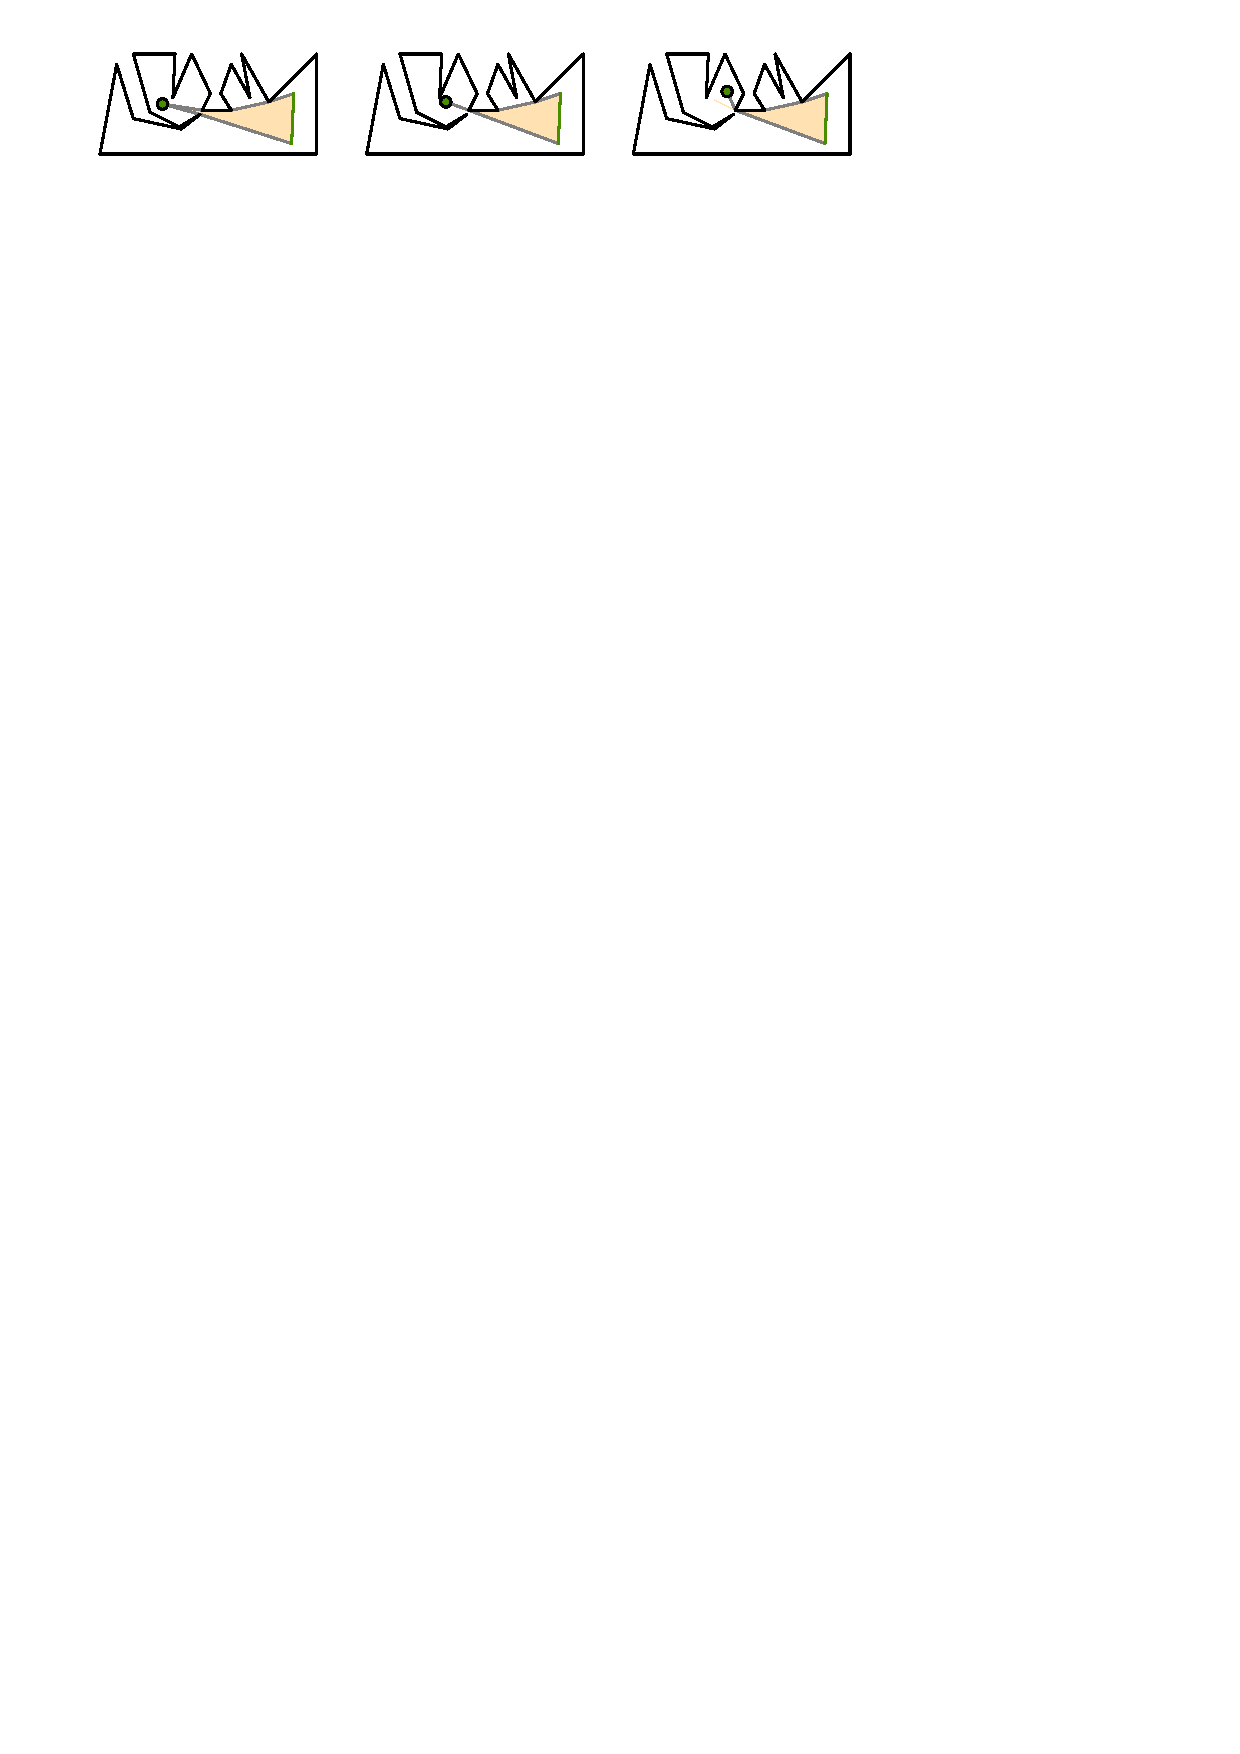
\includegraphics[]{../funnel}
    \caption{Three times a query pair $(q,r)$ in a simple polygon. In the middle case, the paths $\pi_1, \pi_2$ share their first line segment but there still is a point on $r$ which is visible from $q$.}
    \label{fig:funnel}
\end{figure}

\subparagraph{Entity $r$ is contained in a simple polygon.} Consider
the shortest paths $\pi_1, \pi_2$ from $q$ to the end points of
$r$. Observe that if edges of $\pi_1$ and $\pi_2$ coincide, they
coincide in a connected chain from $q$~\cite{guibas1989optimal}. Moreover
(Figure~\ref{fig:funnel}) if more than one line segment of $\pi_1$ and
$\pi_2$ coincide, then any shortest path from $q$ to a point on $r$
cannot be a single line segment. If no edges of $\pi_1$ and $\pi_2$
coincide then there is at least one point on $r$, whose shortest path
to $q$ is a line segment. If exactly one line segment of $\pi_1$
coincides with a segment of $\pi_2$, then that segment must be
connected to $q$ and if there is a line-of-sight between $q$ and $r$,
it has to follow that line segment. This observation allows us to
answer a visibility query by considering only the first three vertices
of $\pi_1$ and $\pi_2$. These vertices can be found in $\O(\log n)$
time using the two-point shortest path data structure of Guibas and
Hershberger~\cite{guibas1989optimal}. We conclude:

% gives us an
% algorithm for the visibility query in this scenario: we simply build
% the shortest path data structure from Guibas and Hershberger which
% takes $\Theta(n)$ space, has $\Theta{O}(n)$ construction and
% $\Theta(\log n)$ query time. Given $q$ and $r$, we use this data
% structure to obtain $\pi_1$ and $\pi_2$ and we check whether the first
% and second edge coincides. If only the first edge coincides we trace
% its supporting line and check if we reach $r$ without intersecting
% $\pi_1$ or $\pi_2$ using their binary tree representation.

\begin{repeattheorem}{thm:one_dead_one_alive}
  Let $P$ be a simple polygon with $n$ vertices. In $\O(n)$ time we
  can build a data structure of size $\O(n)$ with which we can test if
  there is a time at which a stationary entity can see a linearly
  moving entity in $\O(\log n)$ time.
  % We can preprocess a simple polygon $P$ in $\Theta(n)$ space and
  % $\Theta(n)$ time. Such that for any query point $q$ and segment
  % trajectory $r$ which is contained in $P$, we can determine if there
  % is a point on $r$ that is visible from $q$ in $\Theta(\log n)$ time.
\end{repeattheorem}


% \frank{integrate the thing below:}
% \subparagraph{Visibility polygon retrieval.}
% For any point $q$ in a polygonal domain $P$, its \emph{visibility
%   polygon} $V_q$ is the union of all points visible from $q$. 


% A fixed edge coincides with an edge of $P$. An variate edge of $V_q$ is stored as a tuple $(e, v_e)$ where $e$ is an edge and $v_e$ is a vertex of $P$. One endpoint of $e$ is the intersection between the line $qv_e$ and $e$. For all $q \in P$, the \emph{implicit} visibility polygon is a clockwise order of the fixed and variate edges of $V_q$, stored in a red-black tree. Aronov \etal \cite{aronov2002visibility} show how to partition a simple polygon $P$ into $\mathcal{O}(n^2)$ cells such that for each cell, all points in that cell have the same implicit visibility polygon. This allows them to prepreprocess $P$ in $\mathcal{O}(n^2\log n)$ time using $\mathcal{O}(n^2)$ space, such that for any query point $q$, we can get a pointer to the implicit $V_q$ in $\mathcal{O}(\log n)$ time. 
%

\subparagraph{Entity $r$ can cross a simple polygon.}
If $r$ is able to move through edges of $P$ then its trajectory may
intersect the boundary of $P$ linearly often. Inspecting each of the
resulting subsegments explicitly would thus require at least
$\Omega(n)$ time. Hence, we use a different approach.
Let $V_q$ denote the \emph{visibility polygon} of point $q$: the set
of all points visible from $q$. There is a time at which $q$ can see
$r$ if and only if the trajectory of $r$ intersects (the boundary of)
$V_q$. We build a data structure to find such a point (if one
exists).

Aronov~\etal~\cite{aronov2002visibility} actually developed an $\O(n^2)$ size
data structure that can be built in $\O(n^2\log n)$ time and can report the
visibility polygon of an arbitrary query point $q \in P$ in $\O(\log^2 n)$
time. The visibility polygon $V_q$ is returned in its combinatorial
representation, that is, as a (pointer to a) balanced binary search tree,
storing the vertices of $V_q$ in order along the boundary. It is important to
note that this combinatorial representation does not explicitly store the
locations of all vertices of $V_q$. Instead, a vertex $v$ of $V_q$ may be
represented by a pair $(e,w)$, indicating that $v$ is the intersection point of
polygon edge $e$ and the line through vertex $w \in P$ and the query point
$q$. Computing the explicit location of all vertices of $V_q$ thus takes
$\O(|V_q|)$ time, if so desired, by traversing the tree. We now extend the
results of Aronov~\etal in such a way that we can efficiently test if a line
segment intersects $V_q$ \emph{without} spending the $\O(|V_q|)$ time to
compute the explicit locations.

We briefly review the results of Aronov~\etal first. They build a
balanced hierarchical decomposition of
$P$~\cite{Chazelle1989}. Each node $v$ in the balanced
hierarchical decomposition represents a subpolygon $P_v$ of $P$ (the
root corresponds to $P$ itself) and a diagonal of $P_v$ that splits
$P_v$ into two roughly equal size subpolygons $P_\ell$ and $P_r$. For
subpolygon $P_\ell$ the data structure stores a planar subdivision
$\S_\ell$ (of the area outside $P_\ell$) such that for all points in a
cell of $\S_\ell$ the part of the visibility polygon inside $P_\ell$
has the same combinatorial representation. See Figure~\ref{fig:aronov}
for an illustration. Moreover, for each cell it stores the
corresponding combinatorial representation. These representations can
be stored compactly by traversing $\S_\ell$ while maintaining the
(representation of the) visibility polygon in $P_\ell$ in a partially
persistent red black tree~\cite{aronov2002visibility}. The data structure stores an
analogous subdivision for $P_r$. The complete visibility polygon of
$q$ can be obtained by concatenating $\O(\log n)$ subchains of these
pre-stored combinatorial representations (one from every level of the
hierarchical decomposition).

We use the same approach as Aronov~\etal~\cite{aronov2002visibility},
but we use a different representation of $V_q$ (refer to Figure~\ref{fig:twolevel}). Our representation
will be a weight balanced binary search tree
($BB[\alpha]$-tree~\cite{nievergelt1973bbalphatree}) whose leaves
store the vertices of $V_q$ in order along the boundary. An internal
node of this tree corresponds to a subchain of vertices along $V_q$,
which is stored in an associated data structure. We distinguish two
types of vertices in such a chain: \emph{fixed vertices}, for which we
know the exact location, and \emph{variate} vertices, which are
represented by an polygon-edge, polygon-vertex pair $(e,w)$. We store
the fixed vertices in a linear size dynamic data structure that
supports halfspace-emptyness queries, that is, a dynamic convex hull
data structure~\cite{brodal2002dynamic}. This data structure uses $\O(m)$
space, and supports $\O(\log m)$ time updates and queries, where $m$
is the number of stored points. The variate vertices are mapped to a
point in $\R^8$ using a function $f$ that is independent of $q$. We
give the precise definition later. We store the resulting points in a
dynamic data structure that can answer halfspace emptyness
queries~\cite{agarwal1995dynamichalfspace}. This data structure uses
$\O(m\log m)$ space, answers queries in $\O(m^{\frac{3}{4}+\eps})$ time and
supports updates in $\O(\log^2 m)$ time, where $m$ is the number of
points stored. It follows that our representation of $V_q$ uses
$\O(n\log^2 n)$ space, and supports updates in amortized
$\O(\log^3 n)$ time.

% Since (re)building an associated data
% structure of size $m$ takes $O(m\log^2 m)$ time, the total cost for
% rebuilding the associated data structures during rotations in the
% primary tree is $O(n\log^3 n)$~\cite{mehlhorn1984data}.
Since all nodes in the data structure have constant in-degree we can
make it partially persistent at the cost of $\O(\log^3 n)$ space per
update~\cite{driscoll1989persistent}. It follows we can represent the
visibility polygons for all cells in $\S_\ell$ in $O(n^2\log^3 n)$
space.

\begin{figure}[t]
    \centering
    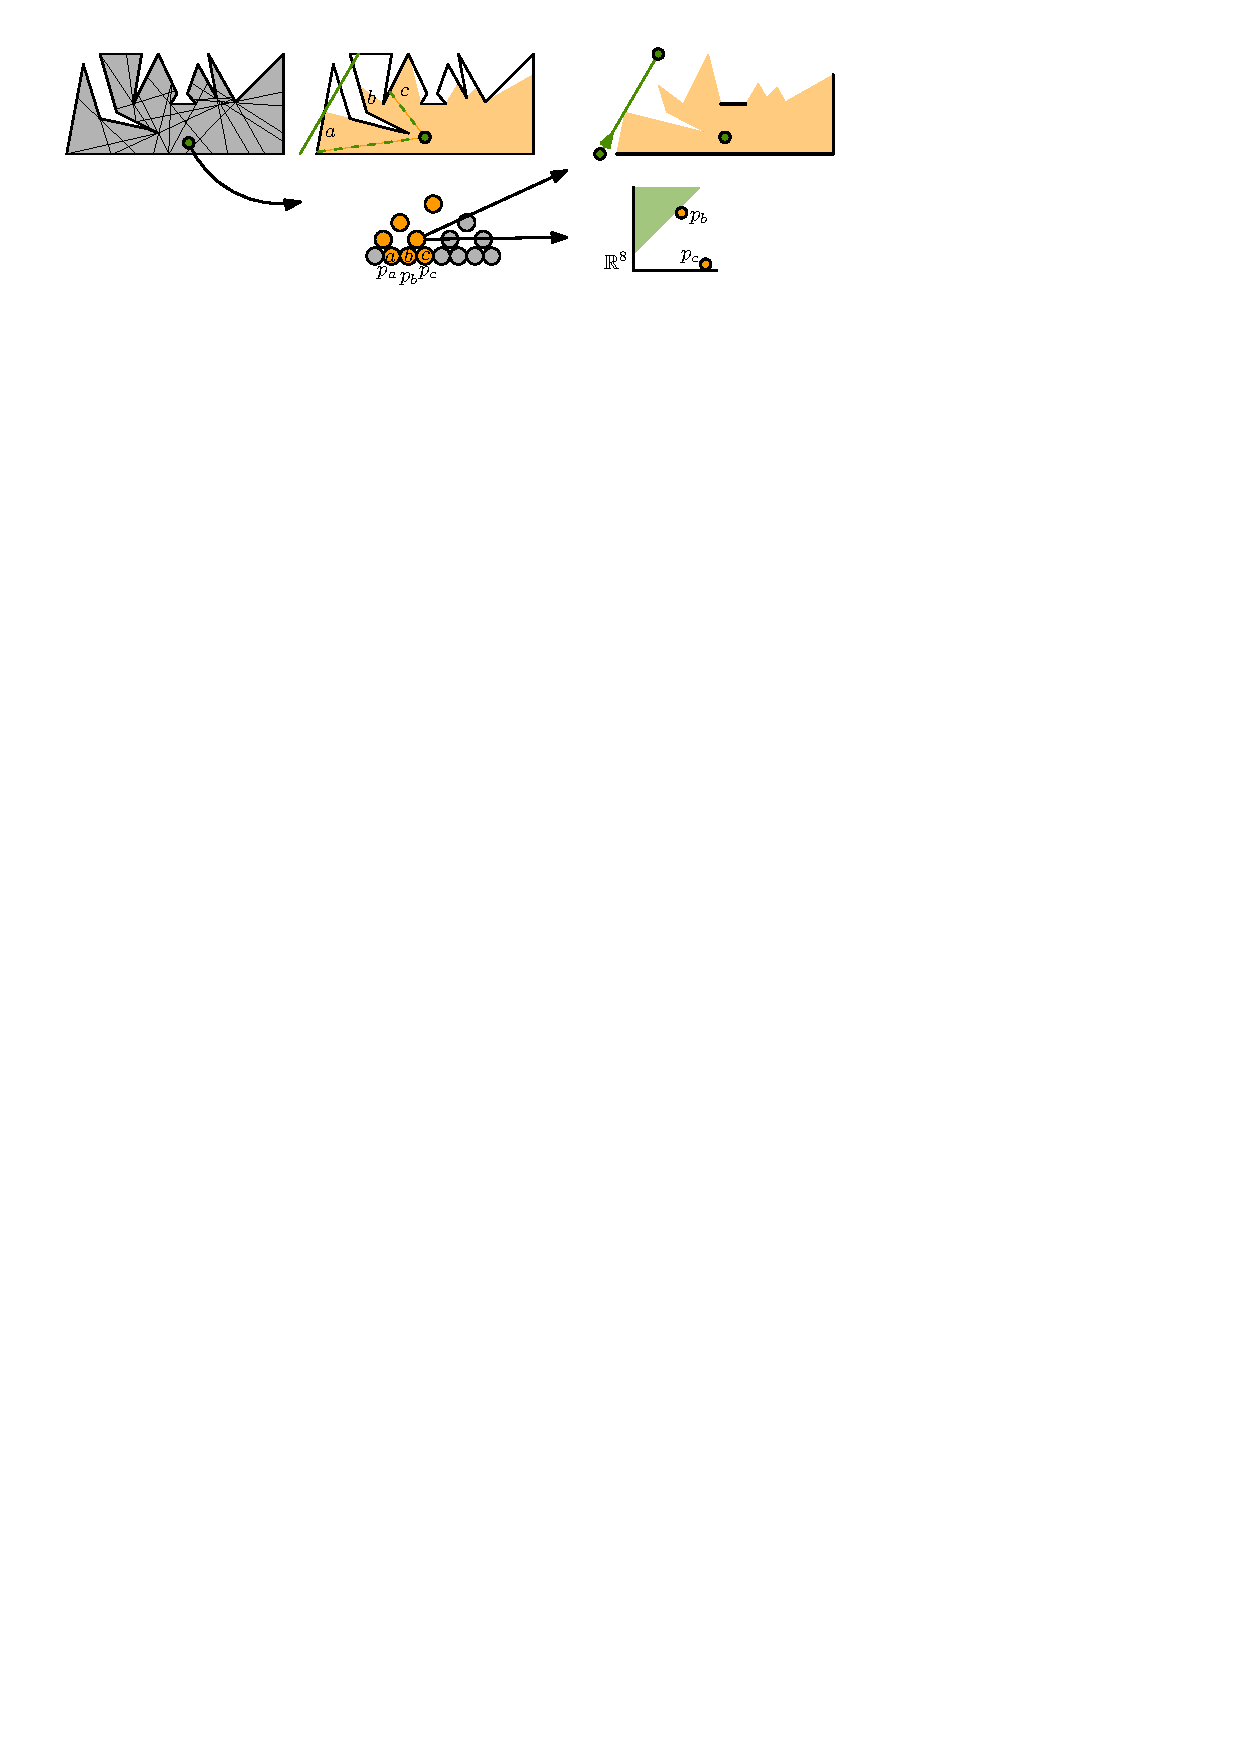
\includegraphics[]{../twolevel}
    \caption{ (left) A simple polygon split in $\mathcal{O}(n^2)$
      cells. For each cell, there exists a red-black tree that
      represents a visibility polygon. (middle) Given $V_q$ and $r$,
      $r$ could intersect the explicit $V_q$ depending on the location
      of $q$. We shoot two rays from $q$ to $r$ and find their
      intersection with $V_q$ in the red-black tree. That gives us
      three leaves highlighted in orange. (right top) All the fixed
      edges in this node are stored in a ray-shooting data structure,
      (right bottom) all the variate edges have 8-dimensional points
      that are stored in an $8$-dimensional partition
      tree.}
    \label{fig:twolevel}
\end{figure}

\subparagraph{Querying.} Given a query $q,r$ we test if the segment $r$
intersects $V_q$. The main idea is to query our data structure for the part of
$V_q$ in the wedge defined by $q$ and $r$. We then extend $r$ into a line $\rho$, and
test if this line separates a vertex of $V_q$ in this wedge from $q$. The
segment $r$ intersects $V_q$, and thus there is a time at which $r$ is visible
from $q$, if and only if this is the case.

We can obtain the part of $V_q$ that lies in the wedge defined by $q$ and $r$,
represented by $O(\log^2 n)$ $BB[\alpha]$-tree nodes. For each of these nodes
we query the associated data structures to test if the halfspace $\rho^{\neg q}$ not
containing $q$ is empty. We can directly query the data structure storing the
fixed vertices with $\rho^{\neg q}$. To test if there is a variate vertex that lies in
$\rho^{\neg q}$ we map it to a halfspace in $\R^8$ using a function $g$.

\begin{lemma}
  \label{lem:query_static}
  There are functions $f$ and $g$ such that $f$ maps each variate vertex
  $(e,w)$ to a point $f(e,w) \in \R^8$ and $g$ maps each $\rho^{\neg q}$ to a
  halfspace $g(\rho^{\neg q})$ in $\R^8$ such that $f(e,w) \in g(\rho^{\neg q})$ if and only
  if the location of the variate vertex $(e,w)$ in $V_q$ lies in $\rho^{\neg q}$.
\end{lemma}

  \begin{figure}[h]
    \centering
    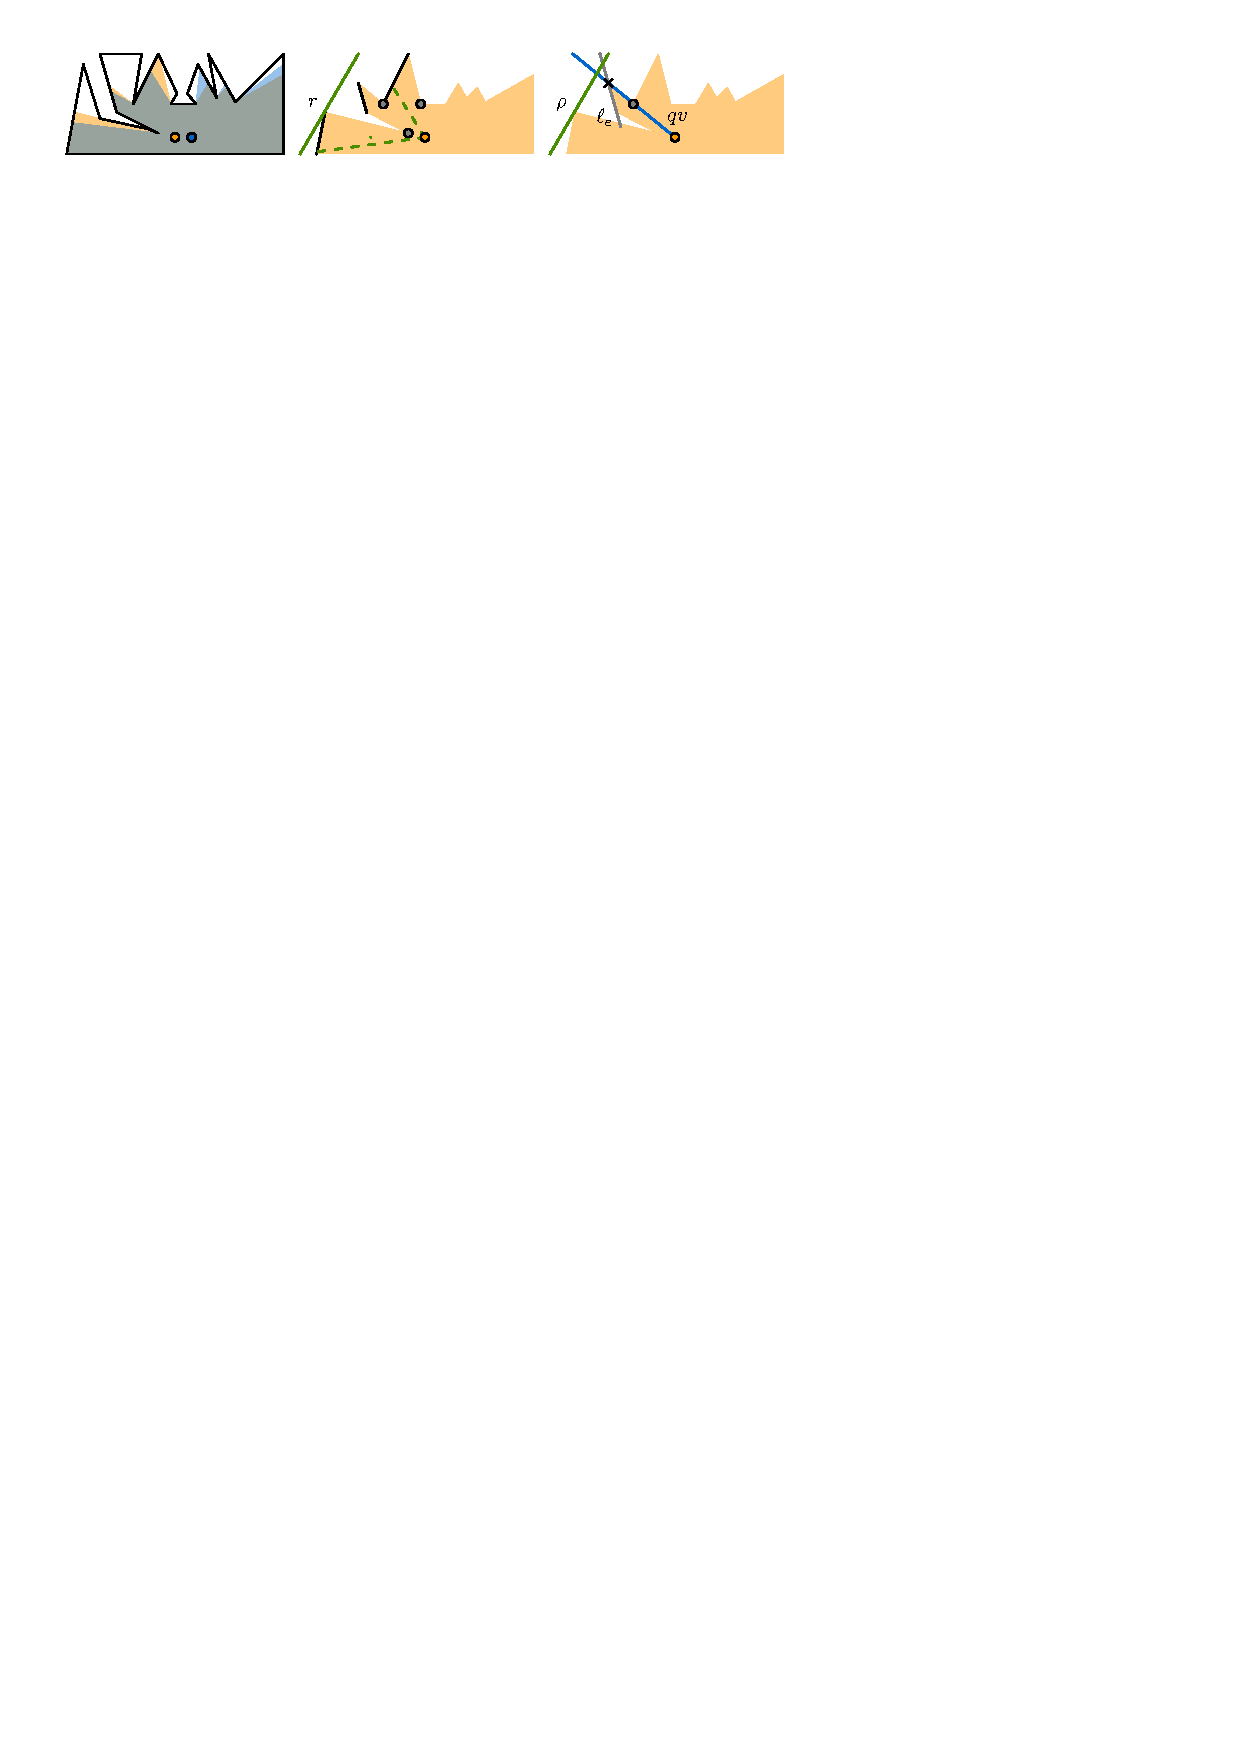
\includegraphics[]{../pointline}
    \caption{ (left) Two points in orange and blue, which have the same implicit visibility polygon, however there could be several placement of $r$ such that $r$ only intersects one of the two explicit visibility polygons. (middle) Entity $r$ in green, $q$ in orange and the chain of uncertain edges. (right) An illustration of the geometric argument. We compute the intersection between $\ell_e$ and $qv$ and check if that point lies below or above $\rho$.}
    \label{fig:pointline}
\end{figure}

\begin{proof}
  Let $q = (a_3,a_4)$, and let $\rho = \{ x,y \mid 0 = a_1 x - a_2 - y \}$ be
  the supporting line of the trajectory of $r$. We describe the construction
  for the case that $q$ lies below $\rho$ and $\rho$ is non-vertical. The other
  cases can be handled analogously.
  
    Refer to Figure~\ref{fig:pointline} (right) for an illustration of the proof.   For each variate vertex $(e,w)$ in a chain we know that the line $qw$  intersects the line $\ell_e$ supporting $e$ on the domain of $e$ (this
  property is guaranteed since $(e,w)$ is a vertex of $V_q$). Moreover, it is
  guaranteed that the intersection point between $qv$ and $\rho$ lies on the
  trajectory of $r$. It follows that $q$ can see $r$ if and only if, the
  intersection point $(x,y)$ between $qw$ and $\ell_e$ lies above $\rho$. Given
  $\rho, q, w$ and $\ell_e$, we can algebraically compute this intersection
  point $(x,y)$. We then substitute the equation for $(x, y)$ into the equation
  for $\rho$ and the point $(x,y)$ lies above this line if and only if the
  result is greater than $0$:

\[
wq := \left\{x,y \mid 0 =  \frac{x_4 - a_4}{x_3 - a_3} x - \frac{x_4 - a_4}{x_3 - a_3}x_3 + x_4  \right\}
\]

The lines $wq$ and $\ell_e$ intersect at the point where their $y$-coordinate is equal and therefore:


\begin{align*}
    x_1 x - x_2 =  \frac{x_4 - a_4}{x_3 - a_3} x - \frac{x_4 - a_4}{x_3 - a_3}x_3 + x_4 \\
    (x_3 - a_3)(x_1 x - x_2) = (x_4 - a_4) x - (x_4 - a_4)x_3 + (x_3 - a_3) x_4 \\
    (x_3 - a_3)x_1 x - (x_4 - a_4) x = x_2 (x_3 - a_3) - (x_4 - a_4)x_3 + (x_3 - a_3) x_4 
\end{align*}


From this equation we can extract the coordinates of the intersection point $(x,y)$ between $wq$ and $\ell_e$:

\begin{align*}
    x = \frac{x_2 (x_3 - a_3) - (x_4 - a_4)x_3 + (x_3 - a_3) x_4}{ (x_3 - a_3)x_1 - (x_4 - a_4)} \\
    y = x_1 \frac{x_2 (x_3 - a_3) - (x_4 - a_4)x_3 + (x_3 - a_3) x_4}{ (x_3 - a_3)x_1 - (x_4 - a_4)} - x_2
\end{align*}

Lastly we substitute the algebraic expression for $(x,y)$ into the formula for $\rho$ and we linearize the predicate:

\begin{align*}
    0 \ge a_1 (x_2 (x_3 - a_3) - (x_4 - a_4)x_3 + (x_3 - a_3) x_4) - \\
    x_2 - x_1 (x_2 (x_3 - a_3) - (x_4 - a_4)x_3 + (x_3 - a_3) x_4) + x_2 \\
    0 \ge [-a_1 a_3] (x_2) + [a_3]( x_1 x_2) + [a_1] (x_2 x_3) + [a_1a_4] (x_3) + \\
    [- a_4] (x_1 x_3) + [- a_1 a_3]( x_4) + [a_3] (x_1 x_4) + [-1](x_1 x_2 x_3)
\end{align*}

Thus we found a predicate $F(\vec{x}, \vec{a})$ with:

\begin{align*}
    (f_1, f_2, f_3, f_4, f_5, f_6, f_6, f_8) = (x_2, x_1x_2, x_2x_3, x_3, x_1x_3, x_4, x_1x_4, x_1x_2x_3) \\
    (g_0, g_1, g_2, g_3, g_4, g_5,g_6, g_7,g_8) = (0, -a_1a_3, a_3, a_1, a_1a_4, -a_4, -a_1a_3, a_3, -1)
\end{align*}

It follows that we can map every variate vertex to a point in $\mathbb{R}^8$
using the $f$-maps provided by the predicate. Any query consisting of the
halfplane $\rho^{\neg q}$ defined by $\rho$ and $q$ gets mapped to a halfspace
in $\mathbb{R}^8$. The half-plane $\rho^{\neg q}$ contains the variate vertex
defined by $q$, $w$, and $e$ if and only if its representative point lies in
this halfspace.
\end{proof}


This theorem now immediately follows:

\begin{repeattheorem}{thm:one_dead_one_ghost}
  Let $P$ be a simple polygon with $n$ vertices. In $O(n^2\log^3 n)$ time We
  can build a data structure of size $O(n^2\log^3 n)$ that can answer
  trajectory visibility queries between a static entity $q$ and a linearly
  moving entity $r$ that may cross $P$ in $O(n^{\frac{3}{4}+\eps})$ time.
\end{repeattheorem}


% \subparagraph{Persistence.}
% The aforementioned data structures create a hierarchical decomposition of $P$ and store in each node of this tree an implicit representation of a sub-polygon of $P$ (be it an hourglass or a visibility polygon) as a red-black tree. A persistent data structure (introduced by Sarnak and Tarjan \cite{sarnak1986planar}) is a data structure that accepts an arbitrarily long sequence of updates, but is able to remember at any time all its earlier versions. Both data structures make use of persistence to save storage space \cite{hershberger1991new, aronov2002visibility}: instead of storing a unique tree at every node of the decomposition they store one partially persistent red-black tree  which for each adjacent node in the decomposition, remembers an update that transforms the red-black tree into the node for that tree.
% %


\subsection{Polygonal domains}
In case $P$ is a polygonal domain we use a
similar approach; we build a subdivision \S in which all points in a cell have
a visibility polygon $V_q$ with the same combinatorial structure, and then
traverse \S while maintaining $V_q$ in a partially persistent data
structure. To obtain \S we simply we simply take all $O(n^2)$ lines defined by
pairs of polygon vertices. The subdivision \S is the arrangement of these lines
and has $O(n^4)$ complexity. We obtain a traversal of \S by computing an Euler
tour of a spanning tree of the dual of \S. We conclude

\begin{repeattheorem}{thm:full_domain}
  Let $P$ be a polygonal domain with $n$ vertices. In $O(n^4\log^3 n)$ time We
  can build a data structure of size $O(n^4\log^3 n)$ that can answer
  trajectory visibility queries between a static entity $q$ and a linearly
  moving entity $r$ that may cross $P$ in $O(n^{\frac{3}{4}+\eps})$ time.
\end{repeattheorem}

\section{Two moving entities in a polygonal domain}
\label{app:Two_moving_entities_in_a_polygonal_domain}

We investigate the two cases where (1) the entities can walk through edges of $P$ and (2) $P$ is a polygonal domain simultaneously. Let $k$ be an unspecified constant. We prove that it is possible to preprocess a polygonal domain $P$ with $n$ vertices in $\mathcal{O}(n^k)$ time, such that for any two entities $q$ and $r$ that each traverse a line segment possibly through edges of $P$, we can determine if there is a moment when $q$ and $r$ are mutually visible in sub-linear time. Our approach almost certainly does not generate an optimal solution with respect to its space requirement and query time. However, it is a non-trivial proof that sub-linear query times are achievable. We obtain these results, by transforming the visibility query in the plane into an intersection query in $\mathbb{R}^4$ and then immediately applying semi-algebraic range searching. 



Let $e_1$ and $e_2$ be two edges of $P$ and denote their visibility glass by $L(e_1, e_2)$. We say that $e_1$ lies on the line $y = x_1 x - x_2$ and $e_2$ lies on the line $y = x_3 x - x_4$. Let $\ell :: y = ax - b$ be a line through $L(e_1, e_2)$ with positive slope and let $e_1$ lie below $e_2$ along $\ell$. The $x$-coordinate of the intersection between $\ell$ and the edges is given by $F_1(a,b) = \frac{b-x_2}{a - x_1}$ and $F_2(a,b) = \frac{b - x_4}{a - x_3}$.

\begin{observation}
Suppose we have a segment on $\ell$ that starts at the point $q$ and ends at the point $r$ then this segment is contained in $L(e_1, e_2)$ if and only if $F_1(a,b) \le x_{q} \le x_{r} \le F_2(a,b)$.
\end{observation}


\begin{figure} [tb]
	\centering 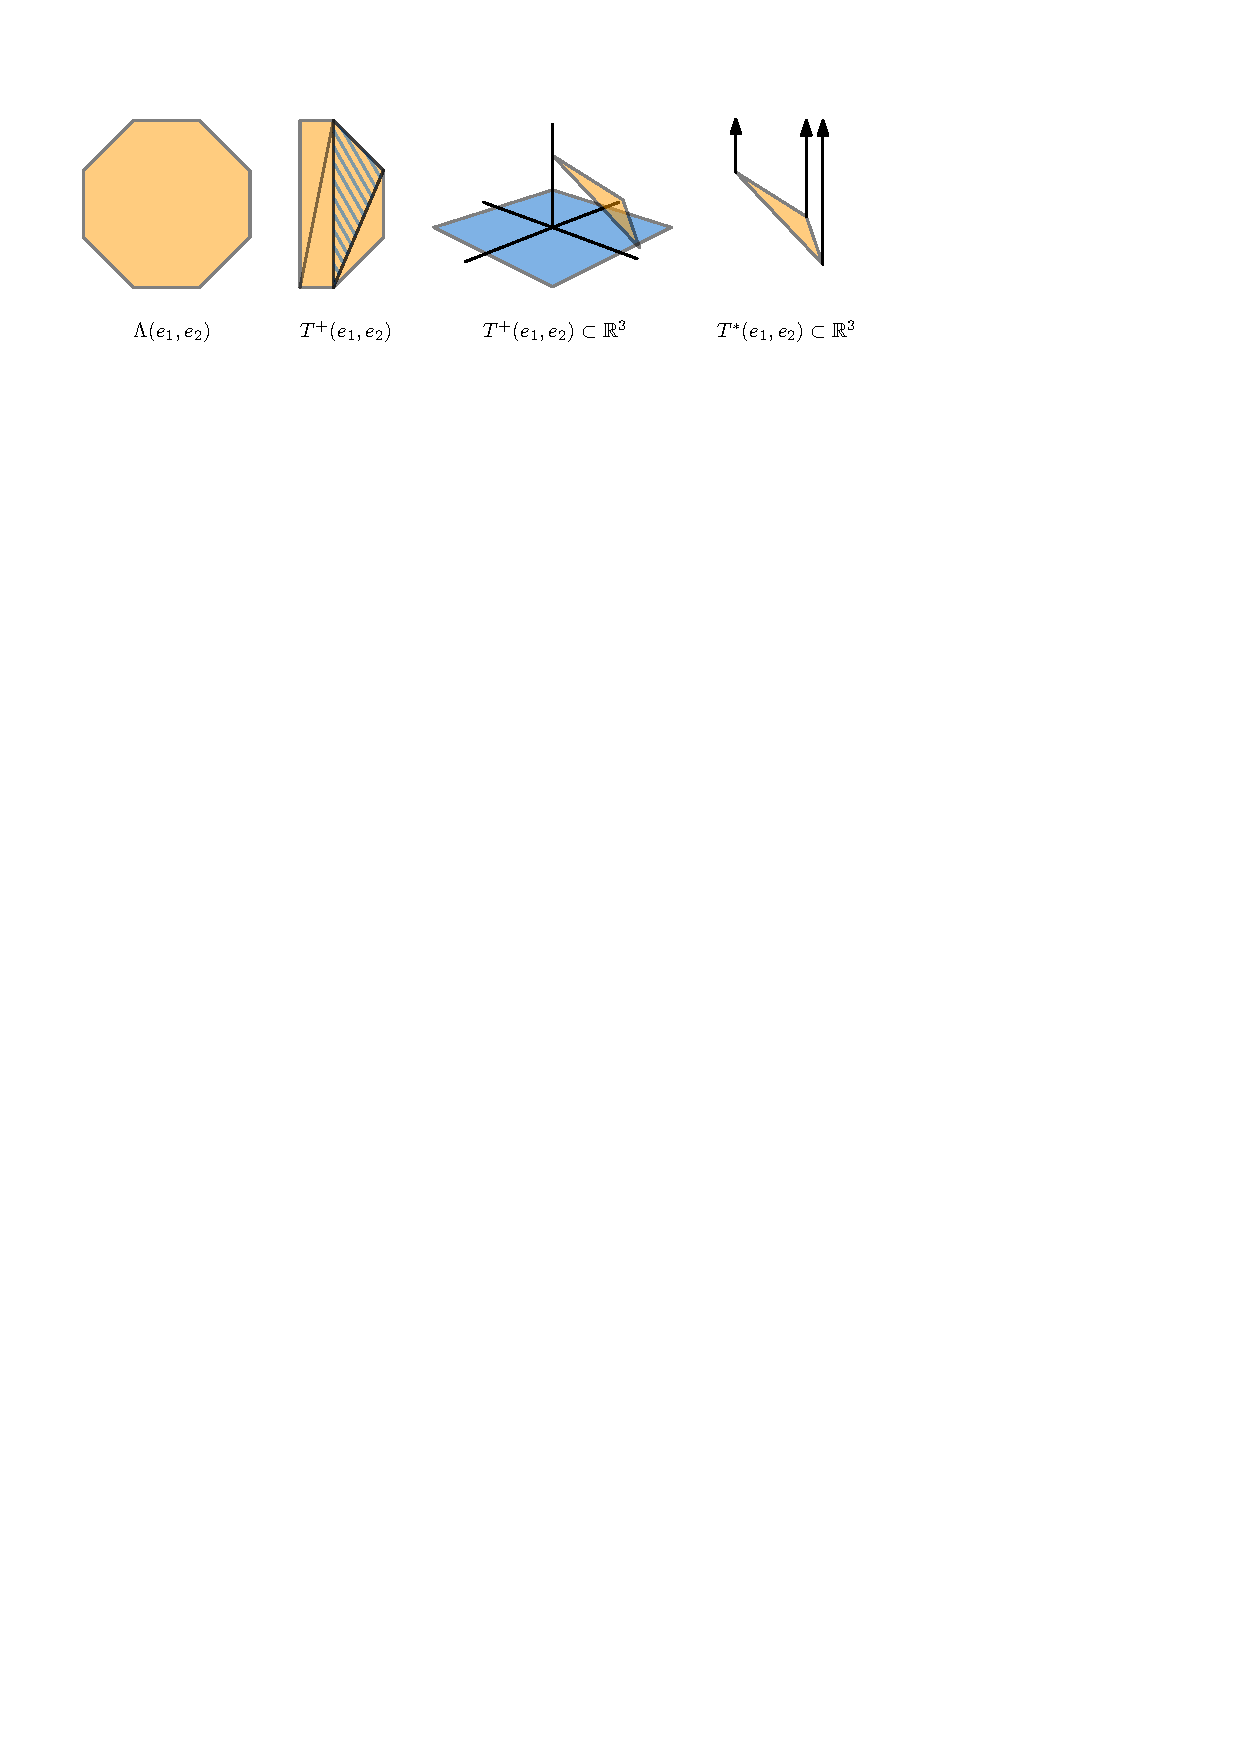
\includegraphics {threedimensional} 
	\caption
	{
	  Unfortunately we cannot draw figures in four dimensions. So we illustrate the mapping from a visibility glass to a three-dimensional volume instead using the map $F_1(a,b)$ based on only the edge $e_1$ and not the edge $e_2$.  
	}  
	\label{fig:threedimensional}
\end{figure}


This observation leads to the following approach for detecting if there is a line-of-sight between $q$ and $r$: we construct for each of the $n^2$ pairs of edges $e_1, e_2$, the two-dimensional area $\Lambda ^+(e_1, e_2)$ which is the dualization of all positive slope lines through the visibility glass between $e_1$ and $e_2$. For reasons that will become apparent later, we triangulate $\Lambda ^+(e_1,e_2)$. Consider any triangle $T^+(e_1, e_2)$ of this triangulation. It represents a collection of positive-slope lines that stab through the visibility glass $L(e_1, e_2)$. We lift $T^+(e_1, e_2)$ to a two-dimensional surface to $\mathbb{R}^4$ with the map that takes a point $(a, b)$ in $T^+(e_1, e_2)$ and that maps it to the point $(a,b, F_1(a,b), F_2(a,b))$. 
This creates a two-dimensional surface in $\mathbb{R}^4$ which has a constant description size. Now consider the following cylinder-like volume in $\mathbb{R}^4$: $T^*(e_1, e_2) = \{ (a,b,c,d) \in \mathbb{R}^4 \mid (a,b,c',d') \in T^+(e_1, e_2) \wedge c' \le c \wedge c \le d \wedge d \le d'  \}$. Any point $(a,b,c,d) \in T^*(e_1, e_2)$, represents a line segment that lies on the line $y = ax-b$, whose start point lies below its end point, and whose start and end point lie between $e_1$ and $e_2$. 
Refer to Figure~\ref{fig:threedimensional} for an example of this transformation in $\mathbb{R}^3$:

Let $q$ and $r$ be given as two line-segment trajectories that do not intersect (if they do intersect, we can always split the visibility query into constantly many visibility queries). Note that we can split $q$ and $r$ into two sub-segments $q'$ and $r'$ where the entity $q$ always has a lower $y$-coordinate than entity $r$ and where the line through $q$ and $r$ has positive slope. We denote by $\gamma'$ the continuous dualization of $q'$ and $r'$ according to equation~\ref{eq:hyperbola}. The two-dimensional curve segment $\gamma'$ can be mapped to a curve segment in $\mathbb{R}^4$ with a mapping that is very similar to our earlier transformation. Each point $(a,b) \in \gamma'$ represents a segment following the line $y = ax - b$ between $q$ and $r$ where $q$ must lie below $r$. We map the point $(a,b)$ to the point $(a,b,c,d)$ where $c$ and $d$ are the $x$-coordinates of intersections of the line $y= ax -b$ with the trajectories of $q$ and $r$ respectively. Coincidentally, this means that we are mapping a point $(a,b)$ to $(a,b, x_{q}, x_{r})$.
If $\gamma'$ intersects $T^*(e_1, e_2)$ then at the time if intersection, the two entities realise a line segment that lies within the visibility glass $L(e_1, e_2)$ and it follows that the entities are mutually visible. Both the volume $T^*$ and the query segment $\gamma'$ can be parametrized with a constant-length parameter, so the predicate that tests their intersection can be linearized to a constant $k$ number of terms.

It follows that we can create a data structure that stores $\mathcal{O}(n^3)$ of these volumes (one for each triangle in both the positive and negative visibility glasses), each represented by a point in $\mathbb{R}^k$. Specifically, we build a cutting tree on these $\mathcal{O}(n^3)$ points in $\mathcal{O}(n^{3k})$ time. A query supplied as two segments $q$ and $r$, can be cut into constantly many pairs of segments where for each pair of segments either $q$ is above $r$ or vice versa. For each pair of segments, we derive its corresponding $k$-dimensional halfspace in $\mathcal{O}(k)$ time and we query the cutting tree in $\mathcal{O}(\log^k n)$ time to see if the halfspace if empty. There is no time when the two entities are mutually visible if and only if each of these queries reports an empty halfspace. Thus we conclude:

\begin{repeattheorem}{thm:polygonal_moving}
  Let $P$ be a polygonal domain with $n$ vertices, and let $k$ be some sufficiently large constant. In $O(n^{3k})$ time we
  can build a data structure of size $O(n^{3k})$ that can answer
  trajectory visibility queries in $\mathcal{O}(\log^k n)$ time.
\end{repeattheorem}


\end{document}
